%%**************************************************************
%% Vorlage fuer Bachelorarbeiten (o.ä.) der DHBW
%%
%% Autor: Tobias Dreher, Yves Fischer
%% Datum: 06.07.2011
%%
%% Autor: Michael Gruben
%% Datum: 15.05.2013
%%
%% Autor: Markus Barthel
%% Datum: 22.08.2014
%%**************************************************************

%!TEX root = ../dokumentation.tex

%
% Nahezu alle Einstellungen koennen hier getaetigt werden
%

\RequirePackage[l2tabu, orthodox]{nag}	% weist in Commandozeile bzw. log auf veraltete LaTeX Syntax hin

\documentclass[%
	pdftex,
	oneside,			% Einseitiger Druck.
	12pt,				% Schriftgroesse
	parskip=half,		% Halbe Zeile Abstand zwischen Absätzen.
%	topmargin = 10pt,	% Abstand Seitenrand (Std:1in) zu Kopfzeile [laut log: unused]
	headheight = 12pt,	% Höhe der Kopfzeile
%	headsep = 30pt,	% Abstand zwischen Kopfzeile und Text Body  [laut log: unused]
	headsepline,		% Linie nach Kopfzeile.
	footsepline,		% Linie vor Fusszeile.
	footheight = 16pt,	% Höhe der Fusszeile
	abstracton,		% Abstract Überschriften
	DIV=calc,		% Satzspiegel berechnen
	BCOR=8mm,		% Bindekorrektur links: 8mm
	headinclude=false,	% Kopfzeile nicht in den Satzspiegel einbeziehen
	footinclude=false,	% Fußzeile nicht in den Satzspiegel einbeziehen
	listof=totoc,		% Abbildungs-/ Tabellenverzeichnis im Inhaltsverzeichnis darstellen
	toc=graphy,	% Literaturverzeichnis im Inhaltsverzeichnis darstellen
]{scrreprt}	% Koma-Script report-Klasse, fuer laengere Bachelorarbeiten alternativ auch: scrbook

% Einstellungen laden
\usepackage{xstring}
\usepackage[utf8]{inputenc}
\usepackage[T1]{fontenc}

\newcommand{\einstellung}[1]{%
  \expandafter\newcommand\csname #1\endcsname{}
  \expandafter\newcommand\csname setze#1\endcsname[1]{\expandafter\renewcommand\csname#1\endcsname{##1}}
}
\newcommand{\langstr}[1]{\einstellung{lang#1}}

\einstellung{matrikelnr}
\einstellung{titel}
\einstellung{kurs}
\einstellung{datumAbgabe}
\einstellung{firma}
\einstellung{firmenort}
\einstellung{abgabeort}
\einstellung{abschluss}
\einstellung{studiengang}
\einstellung{dhbw}
\einstellung{betreuer}
\einstellung{gutachter}
\einstellung{zeitraum}
\einstellung{arbeit}
\einstellung{autor}
\einstellung{sprache}
\einstellung{schriftart}
\einstellung{seitenrand}
\einstellung{kapitelabstand}
\einstellung{spaltenabstand}
\einstellung{zeilenabstand}
\einstellung{zitierstil}
 % verfügbare Einstellungen
%%%%%%%%%%%%%%%%%%%%%%%%%%%%%%%%%%%%%%%%%%%%%%%%%%%%%%%%%%%%%%%%%%%%%%%%%%%%%%%
%                                   Einstellungen
%
% Hier können alle relevanten Einstellungen für diese Arbeit gesetzt werden.
% Dazu gehören Angaben u.a. über den Autor sowie Formatierungen.
%
%
%%%%%%%%%%%%%%%%%%%%%%%%%%%%%%%%%%%%%%%%%%%%%%%%%%%%%%%%%%%%%%%%%%%%%%%%%%%%%%%


%%%%%%%%%%%%%%%%%%%%%%%%%%%%%%%%%%%% Sprache %%%%%%%%%%%%%%%%%%%%%%%%%%%%%%%%%%%
%% Aktuell sind Deutsch und Englisch unterstützt.
%% Es werden nicht nur alle vom Dokument erzeugten Texte in
%% der entsprechenden Sprache angezeigt, sondern auch weitere
%% Aspekte angepasst, wie z.B. die Anführungszeichen und
%% Datumsformate.
\setzesprache{de} % oder en
%%%%%%%%%%%%%%%%%%%%%%%%%%%%%%%%%%%%%%%%%%%%%%%%%%%%%%%%%%%%%%%%%%%%%%%%%%%%%%%%

%%%%%%%%%%%%%%%%%%%%%%%%%%%%%%%%%%% Angaben  %%%%%%%%%%%%%%%%%%%%%%%%%%%%%%%%%%%
%% Die meisten der folgenden Daten werden auf dem
%% Deckblatt angezeigt, einige auch im weiteren Verlauf
%% des Dokuments.
\setzematrikelnr{6526552}
\setzekurs{TINF20ITA}
\setzetitel{Generierung künstlicher Trainingsdaten für die Straßenschilderkennung in Fahrzeugen mittels Generative Adversarial Networks}
\setzedatumAbgabe{08.06.2023}
\setzefirma{}
\setzefirmenort{}
\setzeabgabeort{Stuttgart}
\setzestudiengang{Informatik}
\setzedhbw{Stuttgart}
\setzebetreuer{Prof. Dr. Monika Kochanowski}
\setzezeitraum{24.10.2022 - 08.06.2023}
\setzearbeit{Studienarbeit}
\setzeautor{Frederik Esau}
%%%%%%%%%%%%%%%%%%%%%%%%%%%%%%%%%%%%%%%%%%%%%%%%%%%%%%%%%%%%%%%%%%%%%%%%%%%%%%%%

%%%%%%%%%%%%%%%%%%%%%%%%%%%% Literaturverzeichnis %%%%%%%%%%%%%%%%%%%%%%%%%%%%%%
%% Bei Fehlern während der Verarbeitung bitte in ads/header.tex bei der
%% Einbindung des Pakets biblatex (ungefähr ab Zeile 110,
%% einmal für jede Sprache), biber in bibtex ändern.
\newcommand{\ladeliteratur}{%
\addbibresource{bibliography.bib}
%\addbibresource{weitereDatei.bib}
}
%% Zitierstil
%% siehe: http://ctan.mirrorcatalogs.com/macros/latex/contrib/biblatex/doc/biblatex.pdf (3.3.1 Citation Styles)
%% mögliche Werte z.B numeric-comp, alphabetic, authoryear
\setzezitierstil{ieee}
%%%%%%%%%%%%%%%%%%%%%%%%%%%%%%%%%%%%%%%%%%%%%%%%%%%%%%%%%%%%%%%%%%%%%%%%%%%%%%%%

%%%%%%%%%%%%%%%%%%%%%%%%%%%%%%%%% Layout %%%%%%%%%%%%%%%%%%%%%%%%%%%%%%%%%%%%%%%
%% Verschiedene Schriftarten
% laut nag Warnung: palatino obsolete, use mathpazo, helvet (option scaled=.95), courier instead
\setzeschriftart{libertine} % palatino oder goudysans, lmodern, libertine

%% Paket um Textteile drehen zu können
%\usepackage{rotating}
%% Paket um Seite im Querformat anzuzeigen
%\usepackage{lscape}

%% Seitenränder
\setzeseitenrand{2.5cm}

%% Abstand vor Kapitelüberschriften zum oberen Seitenrand
\setzekapitelabstand{20pt}

%% Spaltenabstand
\setzespaltenabstand{10pt}
%%Zeilenabstand innerhalb einer Tabelle
\setzezeilenabstand{1.5}
%%%%%%%%%%%%%%%%%%%%%%%%%%%%%%%%%%%%%%%%%%%%%%%%%%%%%%%%%%%%%%%%%%%%%%%%%%%%%%%%

%%%%%%%%%%%%%%%%%%%%%%%%%%%%% Verschiedenes  %%%%%%%%%%%%%%%%%%%%%%%%%%%%%%%%%%%
%% Farben (Angabe in HTML-Notation mit großen Buchstaben)
\newcommand{\ladefarben}{%
	\definecolor{LinkColor}{HTML}{00007A}
	\definecolor{ListingBackground}{HTML}{FCF7DE}
}
%% Mathematikpakete benutzen (Pakete aktivieren)
%\usepackage{amsmath}
%\usepackage{amssymb}

%% Programmiersprachen Highlighting (Listings)
\newcommand{\listingsettings}{%
	\lstset{%
		language=Java,			% Standardsprache des Quellcodes
		numbers=left,			% Zeilennummern links
		stepnumber=1,			% Jede Zeile nummerieren.
		numbersep=5pt,			% 5pt Abstand zum Quellcode
		numberstyle=\tiny,		% Zeichengrösse 'tiny' für die Nummern.
		breaklines=true,		% Zeilen umbrechen wenn notwendig.
		breakautoindent=true,	% Nach dem Zeilenumbruch Zeile einrücken.
		postbreak=\space,		% Bei Leerzeichen umbrechen.
		tabsize=2,				% Tabulatorgrösse 2
		basicstyle=\ttfamily\footnotesize, % Nichtproportionale Schrift, klein für den Quellcode
		showspaces=false,		% Leerzeichen nicht anzeigen.
		showstringspaces=false,	% Leerzeichen auch in Strings ('') nicht anzeigen.
		extendedchars=true,		% Alle Zeichen vom Latin1 Zeichensatz anzeigen.
		captionpos=b,			% sets the caption-position to bottom
		backgroundcolor=\color{ListingBackground}, % Hintergrundfarbe des Quellcodes setzen.
		xleftmargin=0pt,		% Rand links
		xrightmargin=0pt,		% Rand rechts
		frame=single,			% Rahmen an
		frameround=ffff,
		rulecolor=\color{darkgray},	% Rahmenfarbe
		fillcolor=\color{ListingBackground},
		keywordstyle=\color[rgb]{0.133,0.133,0.6},
		commentstyle=\color[rgb]{0.133,0.545,0.133},
		stringstyle=\color[rgb]{0.627,0.126,0.941}
	}
}
%%%%%%%%%%%%%%%%%%%%%%%%%%%%%%%%%%%%%%%%%%%%%%%%%%%%%%%%%%%%%%%%%%%%%%%%%%%%%%%%

%%%%%%%%%%%%%%%%%%%%%%%%%%%%%%%% Eigenes %%%%%%%%%%%%%%%%%%%%%%%%%%%%%%%%%%%%%%%
%% Hier können Ergänzungen zur Präambel vorgenommen werden (eigene Pakete, Einstellungen)
\newcommand*\dif{\mathop{}\!\mathrm{d}}
\usepackage{booktabs}
\usepackage{xfrac}
\usepackage{subcaption}
\usepackage{amsmath}
\usepackage{amssymb}
\usepackage{mathtools}
\usepackage{listings}
\usepackage{minted}
\usepackage{caption}
\usepackage{color}
\lstset{backgroundcolor=\color{lightgray}} % lese Einstellungen

\newcommand{\iflang}[2]{%
  \IfStrEq{\sprache}{#1}{#2}{}
}

\langstr{abkverz}
\langstr{anhang}
\langstr{glossar}
\langstr{deckblattabschlusshinleitung}
\langstr{artikelstudiengang}
\langstr{studiengang}
\langstr{anderdh}
\langstr{von}
\langstr{dbbearbeitungszeit}
\langstr{dbmatriknr}
\langstr{dbkurs}
\langstr{dbfirma}
\langstr{dbbetreuer}
\langstr{dbgutachter}
\langstr{sperrvermerk}
\langstr{erklaerung}
\langstr{abstract}
\langstr{listingname}
\langstr{listlistingname}
\langstr{listingautorefname}
 % verfügbare Strings
\input{lang/\sprache} % Übersetzung einlesen

% Einstellung der Sprache des Paketes Babel und der Verzeichnisüberschriften
\iflang{de}{\usepackage[english, ngerman]{babel}}
\iflang{en}{\usepackage[ngerman, english]{babel}} 


%%%%%%% Package Includes %%%%%%%

\usepackage[margin=\seitenrand,foot=1cm]{geometry}	% Seitenränder und Abstände
\usepackage[activate]{microtype} %Zeilenumbruch und mehr
\usepackage[onehalfspacing]{setspace}
\usepackage{makeidx}
\usepackage[autostyle=true,german=quotes]{csquotes}
\usepackage{longtable}
\usepackage{enumitem}	% mehr Optionen bei Aufzählungen
\usepackage{graphicx}
\usepackage{pdfpages}   % zum Einbinden von PDFs
\usepackage{xcolor} 	% für HTML-Notation
\usepackage{float}
\usepackage{array}
\usepackage{calc}		% zum Rechnen (Bildtabelle in Deckblatt)
\usepackage[right]{eurosym}
\usepackage{wrapfig}
\usepackage{pgffor} % für automatische Kapiteldateieinbindung
\usepackage[perpage, hang, multiple, stable]{footmisc} % Fussnoten
\usepackage[printonlyused]{acronym} % falls gewünscht kann die Option footnote eingefügt werden, dann wird die Erklärung nicht inline sondern in einer Fußnote dargestellt
\usepackage{listings}
\usepackage{etoolbox}
\usepackage{svg}

% Notizen. Einsatz mit \todo{Notiz} oder \todo[inline]{Notiz}. 
\usepackage[obeyFinal,backgroundcolor=yellow,linecolor=black]{todonotes}
% Alle Notizen ausblenden mit der Option "final" in \documentclass[...] oder durch das auskommentieren folgender Zeile
% \usepackage[disable]{todonotes}

% Kommentarumgebung. Einsatz mit \comment{}. Alle Kommentare ausblenden mit dem Auskommentieren der folgenden und dem aktivieren der nächsten Zeile.
\newcommand{\comment}[1]{\par {\bfseries \color{blue} #1 \par}} %Kommentar anzeigen
% \newcommand{\comment}[1]{} %Kommentar ausblenden


%%%%%% Configuration %%%%%

%% Anwenden der Einstellungen

\usepackage{\schriftart}
\ladefarben{}

% Titel, Autor und Datum
\title{\titel}
\author{\autor}
\date{\datum}

% PDF Einstellungen
\usepackage[%
	pdftitle={\titel},
	pdfauthor={\autor},
	pdfsubject={\arbeit},
	pdfcreator={pdflatex, LaTeX with KOMA-Script},
	pdfpagemode=UseOutlines, 		% Beim Oeffnen Inhaltsverzeichnis anzeigen
	pdfdisplaydoctitle=true, 		% Dokumenttitel statt Dateiname anzeigen.
	pdflang={\sprache}, 			% Sprache des Dokuments.
]{hyperref}

% (Farb-)einstellungen für die Links im PDF
\hypersetup{
	colorlinks=false, 		% Aktivieren von farbigen Links im Dokument
	linkcolor=LinkColor, 	% Farbe festlegen
	citecolor=LinkColor,
	filecolor=LinkColor,
	menucolor=LinkColor,
	urlcolor=LinkColor,
	%%%%%linktocpage=true, 		% Nicht der Text sondern die Seitenzahlen in Verzeichnissen klickbar
	bookmarksnumbered=true, 	% Überschriftsnummerierung im PDF Inhalt anzeigen.
	pdfborder={0 0 0},
}
% Workaround um Fehler in Hyperref, muss hier stehen bleiben
\usepackage{bookmark} %nur ein latex-Durchlauf für die Aktualisierung von Verzeichnissen nötig

% Schriftart in Captions etwas kleiner
\addtokomafont{caption}{\small}

% Literaturverweise (sowohl deutsch als auch englisch)
\iflang{de}{
\usepackage[
	backend=bibtex,		% empfohlen. Falls biber Probleme macht: bibtex
	bibwarn=true,
	bibencoding=utf8,	% wenn .bib in utf8, sonst ascii
	sortlocale=de_DE,
	style=\zitierstil,
]{biblatex}
}
\iflang{en}{%
\usepackage[
	backend=bibtex,		% empfohlen. Falls biber Probleme macht: bibtex
	bibwarn=true,
	bibencoding=utf8,	% wenn .bib in utf8, sonst ascii
	sortlocale=en_US,
	style=\zitierstil,
]{biblatex}
}

\ladeliteratur{}

% Glossar
\usepackage[nonumberlist,toc]{glossaries}

%%%%%% Additional settings %%%%%%

% Hurenkinder und Schusterjungen verhindern
% http://projekte.dante.de/DanteFAQ/Silbentrennung
\clubpenalty = 10000 % schließt Schusterjungen aus (Seitenumbruch nach der ersten Zeile eines neuen Absatzes)
\widowpenalty = 10000 % schließt Hurenkinder aus (die letzte Zeile eines Absatzes steht auf einer neuen Seite)
\displaywidowpenalty=10000

% Bildpfad
\graphicspath{{images/}}

% Einige häufig verwendete Sprachen
\lstloadlanguages{PHP,Python,Java,C,C++,bash}
\listingsettings{}
% Umbennung des Listings
\renewcommand\lstlistingname{\langlistingname}
\renewcommand\lstlistlistingname{\langlistlistingname}
\def\lstlistingautorefname{\langlistingautorefname}

% Abstände in Tabellen
\setlength{\tabcolsep}{\spaltenabstand}
\renewcommand{\arraystretch}{\zeilenabstand}

%%%%% IMPORTIERTER CODE %%%%%%%%%%%%%%%%%%%
\newcommand{\mkbibnodate}{o\adddot D\adddot} %%%%% BZW {n\adddot d\adddot} WENN AUF EGNLISCH
\AtEveryCitekey{\iffieldundef{labelyear}{\restorefield{labelyear}{\mkbibnodate}}{}}
\AtEveryBibitem{\iffieldundef{year}{\restorefield{year}{\mkbibnodate}}{}}

\DeclareSourcemap{
	\maps[datatype=bibtex]{
		\map[overwrite=false]{
			\step[fieldset=date,origfieldval,final]
			\step[fieldset=eventdate,origfieldval,final]
			\step[fieldset=origdate,origfieldval,final]
			\step[fieldset=urldate,origfieldval,final]
			\step[fieldset=eventyear,origfieldval,final]
			\step[fieldset=origyear,origfieldval,final]
			\step[fieldset=urlyear,origfieldval,final]
			\step[fieldset=year,fieldvalue={o.D.},final] %%%% BZW n.d. WENN AUF ENGLISCH
			\step[fieldset=sortyear,fieldvalue={0000}]
		}
	}
}
%%%%% ENDE IMPORTIERTER CODE %%%%%%%%%%%%%%

\makeglossaries
%!TEX root = ../dokumentation.tex

%
% vorher in Konsole folgendes aufrufen:
%	makeglossaries makeglossaries dokumentation.acn && makeglossaries dokumentation.glo
%

%
% Glossareintraege --> referenz, name, beschreibung
% Aufruf mit \gls{...}
%
\newglossaryentry{Glossareintrag}{name={Glossareintrag},,description={Ein Glossar beschreibt verschiedenste Dinge in kurzen Worten}}
\newglossaryentry{weight}{name=Weight, description={Gewicht}}


\begin{document}

	% Deckblatt
	\begin{spacing}{1}
		%!TEX root = ../dokumentation.tex

\begin{titlepage}
	\begin{center}
		%{\raisebox{\ht\strutbox-(\totalheight*2)}{\includegraphics[width=50mm,scale=0.5]{images/CLAAS low res.png}}} &
		%%%%%{\raisebox{0cm}{\includegraphics[width=50mm,scale=0.5]{images/CLAAS low res.png}}} &
		
\includegraphics[height=2.5cm]{images/dhbw.png}
	\end{center}
	\enlargethispage{20mm}
	\begin{center}
		\vspace*{12mm}	{\LARGE\textbf \titel }\\
		\vspace*{12mm}	{\large\textbf{\arbeit}}\\
		%\vspace*{12mm}	\langdeckblattabschlusshinleitung\\
		%\vspace*{3mm}		{\textbf \abschluss}\\
		\vspace*{12mm}	\langstudiengang{} \studiengang\\
    \vspace*{3mm}		\langanderdh{} \dhbw\\
		\vspace*{12mm}	\langvon\\
		\vspace*{3mm}		{\large\textbf \autor}\\
		\vspace*{12mm}	\datumAbgabe\\
	\end{center}
	\vfill
	\begin{spacing}{1.2}
	\begin{tabbing}
		mmmmmmmmmmmmmmmmmmmmmmmmmm             \= \kill
		\textbf{\langdbbearbeitungszeit}       \>  \zeitraum\\
		\textbf{\langdbmatriknr, \langdbkurs}  \>  \matrikelnr, \kurs\\
		\textbf{\langdbbetreuer}               \>  \betreuer\\
		%\textbf{\langdbgutachter}              \>  \gutachter
	\end{tabbing}
	\end{spacing}
\end{titlepage}

	\end{spacing}
	\newpage

	\pagenumbering{Roman}

	% Sperrvermerk
	%%%!TEX root = ../dokumentation.tex

\thispagestyle{empty}
% Sperrvermerk direkt hinter Titelseite
\section*{\langsperrvermerk}

\vspace*{2em}

\iflang{de}{%
  Der Inhalt dieser Arbeit darf weder als Ganzes noch in Auszügen Personen
außerhalb des Prüfungsprozesses und des Evaluationsverfahrens zugänglich gemacht werden,
sofern keine anderslautende Genehmigung der Ausbildungsstätte vorliegt.
}

%http://www.ib.dhbw-mannheim.de/fileadmin/ms/bwl-ib/Downloads_alt/Leitfaden_31.05.pdf

\iflang{en}{%
  The {\arbeit} on hand 
  \begin{center}{\itshape{} \titel{}\/}\end{center} 
   contains internal resp.\ confidential data of {\firma}. It is intended solely for inspection by the assigned examiner, the head of the {\studiengang} department and, if necessary, the Audit Committee \langanderdh{} {\dhbw}. It is strictly forbidden
    \begin{itemize}
    \item to distribute the content of this paper (including data, figures, tables, charts etc.) as a whole or in extracts,
    \item to make copies or transcripts of this paper or of parts of it,
    \item to display this paper or make it available in digital, electronic or virtual form.
    \end{itemize}
  Exceptional cases may be considered through permission granted in written form by the author and {\firma}.
}

\vspace{3em}

\abgabeort, \datumAbgabe
\vspace{4em}

\rule{6cm}{0.4pt}\\
\autor

	%%\newpage

	% Erklärung
	%!TEX root = ../dokumentation.tex

\thispagestyle{empty}

\section*{\langerklaerung}
\vspace*{2em}

\iflang{de}{%
Ich versichere hiermit, dass ich meine {\arbeit} mit dem Thema: {\itshape \titel } selbstständig verfasst und keine anderen als die angegebenen Quellen und Hilfsmittel benutzt habe. Ich versichere zudem, dass die eingereichte elektronische Fassung mit der gedruckten Fassung übereinstimmt. 

% https://www.dhbw-karlsruhe.de/fileadmin/user_upload/dokumente/T-Informatik/Prüfungsordnung-Technik-2015-09-29.pdf (S. 19)
% https://www.dhbw-stuttgart.de/fileadmin/dateien/Amtliche_Bekanntmachungen/20_2017_Bekanntmachung_StuPrO_DHBW_Technik.pdf (S. 21)


% Ich erkläre hiermit ehrenwörtlich: \\
% \begin{enumerate}
% \item dass ich meine {\arbeit} mit dem Thema
% {\itshape \titel } ohne fremde Hilfe angefertigt habe;
% \item dass ich die Übernahme wörtlicher Zitate aus der Literatur sowie die Verwendung der Gedanken
% anderer Autoren an den entsprechenden Stellen innerhalb der Arbeit gekennzeichnet habe;
% \item dass ich meine {\arbeit} bei keiner anderen Prüfung vorgelegt habe;
% \item dass die eingereichte elektronische Fassung exakt mit der eingereichten schriftlichen Fassung
% übereinstimmt.
% \end{enumerate}
% 
% Ich bin mir bewusst, dass eine falsche Erklärung rechtliche Folgen haben wird.

% % http://www.ib.dhbw-mannheim.de/fileadmin/ms/bwl-ib/Downloads_alt/Leitfaden_31.05.pdf (S. 52)
}


\iflang{en}{%
Hereby I solemnly declare:
\begin{enumerate}
\item that this {\arbeit}, titled {\itshape \titel } is entirely the product of my own scholarly work, unless otherwise indicated in the text or references, or acknowledged below;
\item I have indicated the thoughts adopted directly or indirectly from other sources at the appropriate places within the document;
\item this {\arbeit} has not been submitted either in whole or part, for a degree at this or any other university or institution;
\item I have not published this {\arbeit} in the past; 
\item the printed version is equivalent to the submitted electronic one.
\end{enumerate}
I am aware that a dishonest declaration will entail legal consequences.
}

\vspace{3em}

\abgabeort, \datumAbgabe
\vspace{4em}

\rule{6cm}{0.4pt}\\
\autor

	\newpage

	% Abstract
	%!TEX root = ../dokumentation.tex

\pagestyle{empty}

\iflang{de}{%
% Dieser deutsche Teil wird nur angezeigt, wenn die Sprache auf Deutsch eingestellt ist.
\renewcommand{\abstractname}{\langabstract} % Text für Überschrift

% \begin{otherlanguage}{english} % auskommentieren, wenn Abstract auf Deutsch sein soll
\begin{abstract}
Abstract normalerweise auf Englisch. Siehe:  \url{http://www.dhbw.de/fileadmin/user/public/Dokumente/Portal/Richtlinien_Praxismodule_Studien_und_Bachelorarbeiten_JG2011ff.pdf} (8.3.1 Inhaltsverzeichnis)

Ein "`Abstract"' ist eine prägnante Inhaltsangabe, ein Abriss ohne Interpretation und Wertung einer wissenschaftlichen Arbeit. In DIN 1426 wird das (oder auch der) Abstract als Kurzreferat zur Inhaltsangabe beschrieben.

\begin{description}
\item[Objektivität] soll sich jeder persönlichen Wertung enthalten
\item[Kürze] soll so kurz wie möglich sein
\item[Genauigkeit] soll genau die Inhalte und die Meinung der Originalarbeit wiedergeben
\end{description}

Üblicherweise müssen wissenschaftliche Artikel einen Abstract enthalten, typischerweise von 100-150 Wörtern, ohne Bilder und Literaturzitate und in einem Absatz.

Quelle: \url{http://de.wikipedia.org/wiki/Abstract} Abgerufen 07.07.2011

Diese etwa einseitige Zusammenfassung soll es dem Leser ermöglichen, Inhalt der Arbeit und Vorgehensweise
des Autors rasch zu überblicken. Gegenstand des Abstract sind insbesondere 
\begin{itemize}
\item Problemstellung der Arbeit,
\item im Rahmen der Arbeit geprüfte Hypothesen bzw. beantwortete Fragen,
\item der Analyse zugrunde liegende Methode,
\item wesentliche, im Rahmen der Arbeit gewonnene Erkenntnisse,
\item Einschränkungen des Gültigkeitsbereichs (der Erkenntnisse) sowie nicht beantwortete Fragen. 
\end{itemize}
Quelle: \url{http://www.ib.dhbw-mannheim.de/fileadmin/ms/bwl-ib/Downloads_alt/Leitfaden_31.05.pdf}, S.~49
\end{abstract}
% \end{otherlanguage} % auskommentieren, wenn Abstract auf Deutsch sein soll
}



\iflang{en}{%
% Dieser englische Teil wird nur angezeigt, wenn die Sprache auf Englisch eingestellt ist.
\renewcommand{\abstractname}{\langabstract} % Text für Überschrift

\begin{abstract}
An abstract is a brief summary of a research article, thesis, review, conference proceeding or any in-depth analysis of a particular subject or discipline, and is often used to help the reader quickly ascertain the paper's purpose. When used, an abstract always appears at the beginning of a manuscript, acting as the point-of-entry for any given scientific paper or patent application. Abstracting and indexing services for various academic disciplines are aimed at compiling a body of literature for that particular subject.

The terms précis or synopsis are used in some publications to refer to the same thing that other publications might call an ``abstract''. In ``management'' reports, an executive summary usually contains more information (and often more sensitive information) than the abstract does.

Quelle: \url{http://en.wikipedia.org/wiki/Abstract_(summary)}

\end{abstract}
}
	\newpage %\sqrt{}

	\pagestyle{plain}		% nur Seitenzahlen im Fuß
	
	\RedeclareSectionCommand[beforeskip=\kapitelabstand         ]{chapter} % stellt Abstand vor Kapitelüberschriften ein

	% Inhaltsverzeichnis
	\begin{spacing}{1.1}
		\begingroup
		
			% auskommentieren für Seitenzahlen unter Inhaltsverzeichnis
			\renewcommand*{\chapterpagestyle}{empty}
			\pagestyle{empty}
			
			
			\setcounter{tocdepth}{2}
			%für die Anzeige von Unterkapiteln im Inhaltsverzeichnis
			%\setcounter{tocdepth}{2}
			
			\tableofcontents
			\clearpage
		\endgroup
	\end{spacing}
	\newpage

	% Abkürzungsverzeichnis
	\cleardoublepage
	%!TEX root = ../dokumentation.tex

\addchap{Abkürzungsverzeichnis}
%nur verwendete Akronyme werden letztlich im Abkürzungsverzeichnis des Dokuments angezeigt
%Verwendung: 
%		\ac{Abk.}   --> fügt die Abkürzung ein, beim ersten Aufruf wird zusätzlich automatisch die ausgeschriebene Version davor eingefügt bzw. in einer Fußnote (hierfür muss in header.tex \usepackage[printonlyused,footnote]{acronym} stehen) dargestellt
%		\acs{Abk.}   -->  fügt die Abkürzung ein
%		\acf{Abk.}   --> fügt die Abkürzung UND die Erklärung ein
%		\acl{Abk.}   --> fügt nur die Erklärung ein
%		\acp{Abk.}  --> gibt Plural aus (angefügtes 's'); das zusätzliche 'p' funktioniert auch bei obigen Befehlen
%	siehe auch: http://golatex.de/wiki/%5Cacronym
%	

%%%%%%%%%%%%%%%% IMPORTIERTER CODE %%%%%%%%%%%%%%%%%%%%%%%%%%%%%%%
% provides \AtBeginEnvironment, \patchcmd and \csdef:

\makeatletter
\newcommand{\acroforeign}[1]{}

% patch the environment to print the foreign definition:
\AtBeginEnvironment{acronym}{%
	\def\acroforeign#1{ (#1)}%
}

% patch the acronym definition to safe the foreign definition:
\expandafter\patchcmd\csname AC@\AC@prefix{}@acro\endcsname
{\begingroup}
{\begingroup\def\acroforeign##1{\csdef{ac@#1@foreign}{##1, }}}
{}
{\fail}

% %   renew the first output to include the foreign definition if given:
\renewcommand*{\@acf}[2][\AC@linebreakpenalty]{%
	\ifAC@footnote
	\acsfont{\csname ac@#2@foreign\endcsname\AC@acs{#2}}%
	\footnote{\AC@placelabel{#2}\AC@acl{#2}{}}%
	\else
	\acffont{%
		\AC@placelabel{#2}\AC@acl{#2}%
		\nolinebreak[#1] %
		\acfsfont{(\acsfont{\csname ac@#2@foreign\endcsname\AC@acs{#2}})}%
	}%
	\fi
	\ifAC@starred\else\AC@logged{#2}\fi
}
\makeatother
%%%%%%%%%%%%%%%%%%%%%%%%%% ENDE IMPORTIERTER CODE %%%%%%%%%%%%%%%%%%%%%%

\begin{acronym}[AUTOSAR]
	%\setlength{\itemsep}{-\parsep}
	\acro{CNN}{Convolutional Neural Network}
	\acro{CycleGAN}{Cycle-Consistent Generative Adversarial Network}
	\acro{GAN}{Generative Adversarial Network}
	\acro{GTSRB}{German Traffic Sign Recognition Benchmark}
	\acro{KNN}{Künstliches Neuronales Netz}
	\acro{LSTM}{Long Short-term Memory}
	\acro{PixelRNN}{Pixel Recurrent Neural Network}
\end{acronym}


	% Abbildungsverzeichnis
	\cleardoublepage
	\listoffigures

	% Tabellenverzeichnis
	\cleardoublepage
	\listoftables

	% Quellcodeverzeichnis
	\cleardoublepage
	\lstlistoflistings
	\cleardoublepage

	\pagenumbering{arabic}
	
	\pagestyle{headings}		% Kolumnentitel im Kopf, Seitenzahlen im Fuß

	% Inhalt
	%%%%%\foreach \i in {01,02,03,04,05,06,07,08,09,...,99} {%
	%%%%%	\edef\FileName{content/\i kapitel}%
	%%%%%		\IfFileExists{\FileName}{%
	%%%%%			\input{\FileName}
	%%%%%		}
	%%%%%		{%
	%%%%%			%file does not exist
	%%%%%		}
	%%%%%}

	\chapter{Einleitung}
Während in großen Teilen des letzten Jahrhunderts Innovationen in der Fahrzeugentwicklung vor allem im Bereich der mechanischen Leistung und Effizienz stattgefunden haben, erwartet man zukünftige Verbesserungen im Automobil besonders softwareseitig \cite{Staron2021}. ... 
\section{Problemstellung}

\section{Vorgehensweise}
\section{Ziel der Arbeit}
	\chapter{Stand der Technik}
\section{Straßenschilderkennung}
\label{chap:stand-der-technik-strassenschilderkennung}
Eine Straßenschilderkennung zählt mittlerweile zu der Standardausstattung vieler Neuwagen. Im Jahr 2024 tritt zudem eine EU-Verordnung in Kraft, durch die sämtliche neu produzierten Fahrzeuge mit einer solchen Funktion ausgestattet werden müssen \cite{eu-regulation}. Daran zeigt sich, dass das Thema bereits weitreichend etabliert ist.

Straßenschilder werden zu folgendem Zweck eingesetzt: Es sollen Informationen über die Verkehrssituation und über geltende Vorschriften des Gebiets, in dem sich das Fahrzeug zu einem gegebenen Zeitpunkt befindet, präsentiert werden. Durch Straßenschilder werden unter anderem Geschwindigkeitsvorgaben, Gefahrenhinweise und allgemeine Verkehrsregeln kommuniziert. Dabei sind die Schilder so konzipiert, dass sie sich visuell möglichst von ihrem Hintergrund abheben und leicht voneinander zu unterscheiden sind. Automatische Straßenschilderkennungen können Fahrer*innen in Situationen unterstützen, in denen sie Schilder übersehen oder gezielt missachten. Anstelle dass ein reales Schild beispielsweise nur für einige Sekunden sichtbar ist, bevor es außerhalb der Sichtweite des Fahrzeugführenden ist, ist eine durchgehende Anzeige auf den Displays eines Fahrzeugs möglich. Auch akustische Warnungen oder ein aktives Eingreifen von Sicherheitssystemen sind denkbar, beziehungsweise bereits in Serienfahrzeugen vorhanden.

Eine Straßenschilderkennung erfolgt visuell und wird somit mittels Kameras umgesetzt. Dabei lassen sich viele Schilder durch eine bestimmte Form (Kreis, Dreieck, Achteck, etc.) und ein Piktogramm (Schneeflocke, Person, etc.) oder eine Zahl identifizieren. Somit können die verschiedenen Arten von Straßenschilder in Klassen unterteilt werden, die durch den Erkennungsalgorithmus detektiert werden. Für die praktische Umsetzung solcher Algorithmen werden häufig \acp{KNN} verwendet. Diese werden in Kapitel \ref{chap:KNNs} thematisch aufgeführt. Besonders relevant für das Thema dieser Studienarbeit ist, wie zuverlässig die momentan ausgelieferten Straßenschilderkennungen sind und welche Situationen die Algorithmen am ehesten zu falschen Aussagen verleiten. Auf dieser Grundlagen kann sich orientiert werden, welche Arten von Bildern vermehrt generiert werden sollen, um die Straßenschilderkennung verbessern zu können.

Im Jahr 2019 hat eine Automobilzeitschrift die Straßenschilderkennung von unterschiedlichen Fahrzeugherstellern getestet \cite{strassenschilderkennungTest}. Zudem existieren verschiedene Publikationen, die sich mit der Thematik befassen \cite{traffic-sign-detection-review-2014}. Die Ergebnisse des Zeitschriftenartikels weisen darauf hin, dass die Straßenschilderkennung einiger Fahrzeuger bereits weitreichend funktioniert. Geschwindigkeitsvorgaben werden überwiegend erkannt und dem Fahrer auf einem Display angezeigt. Auch existieren bereits akustische Warnungen bei einer Überschreitung der Höchstgeschwindigkeit. Dennoch existieren einige Situationen, die bei mehreren Fahrzeugen zu Problemen bei der Straßenschilderkennung geführt haben. Einen exemplarischen Überblick soll die folgende Grafik bieten: \cite{strassenschilderkennungTest} 

\begin{figure}[H]
   \centering
   \captionsetup[subfigure]{labelformat=empty}
   \begin{subfigure}[b]{0.125\textwidth}
       \centering
       
\includegraphics[height=\textwidth]{../images/Schilder Beispiele/Aufhebungsschild.png}
       \caption{Aufhebung}
       \label{fig:aufhebungsschild}
   \end{subfigure}
   \hspace{3em}%
   \begin{subfigure}[b]{0.125\textwidth}
       \centering
       
\includegraphics[height=\textwidth]{../images/Schilder Beispiele/Abgeklebt.jpg}
       \caption{Ungültigkeit}
       \label{fig:abgeklebt}
   \end{subfigure}
   \hspace{3em}%
   \begin{subfigure}[b]{0.125\textwidth}
       \centering
       
\includegraphics[height=\textwidth]{../images/Schilder Beispiele/Dunkelheit.png}
       \caption{Dunkelheit}
       \label{fig:dunkelheit}
   \end{subfigure}
   \hspace{3em}%
   \begin{subfigure}[b]{0.125\textwidth}
    \centering
    
\includegraphics[height=\textwidth]{../images/Schilder Beispiele/Wechselverkehrszeichen.jpg}
    \caption{LED Schilder}
    \label{fig:ledschild}
   \end{subfigure}
      \caption{Erschwerende Einflüsse auf die Straßenschilderkennung}
      \label{fig:einfluesse-strscherkennung}
\end{figure}

Fahrzeuge verschiedener Hersteller haben in den Tests Aufhebungsschilder nicht korrekt interpretiert. Damit sind Schilder gemeint, die entweder Geschwindigkeitsbegrenzungen oder Überholverbote außer Kraft setzen. Des Weiteren sorgten mittels Klebestreifen als ungültig erklärte Schilder, in einigen Fällen Dunkelheit, beispielsweise in Tunneln, und sogenannte LED \emph{Wechselverkehrszeichen} für falsche Aussagen. Auch wird teilweise nicht erkannt, wenn Schilder für eine kreuzende Straße gelten, statt für die Straße, auf der sich das Fahrzeug zu dem gebenen Zeitpunkt befinden. Weitere Aspekte, die in dem Artikel nicht explizit genannt sind, aber laut einer Publikation von 2014 in der Vergangenheit zu Schwierigkeiten geführt haben, sind mitunter die folgenden: \cite{traffic-sign-detection-review-2014}

\begin{figure}[H]
   \centering
   \captionsetup[subfigure]{labelformat=empty}
   \begin{subfigure}[b]{0.125\textwidth}
       \centering
       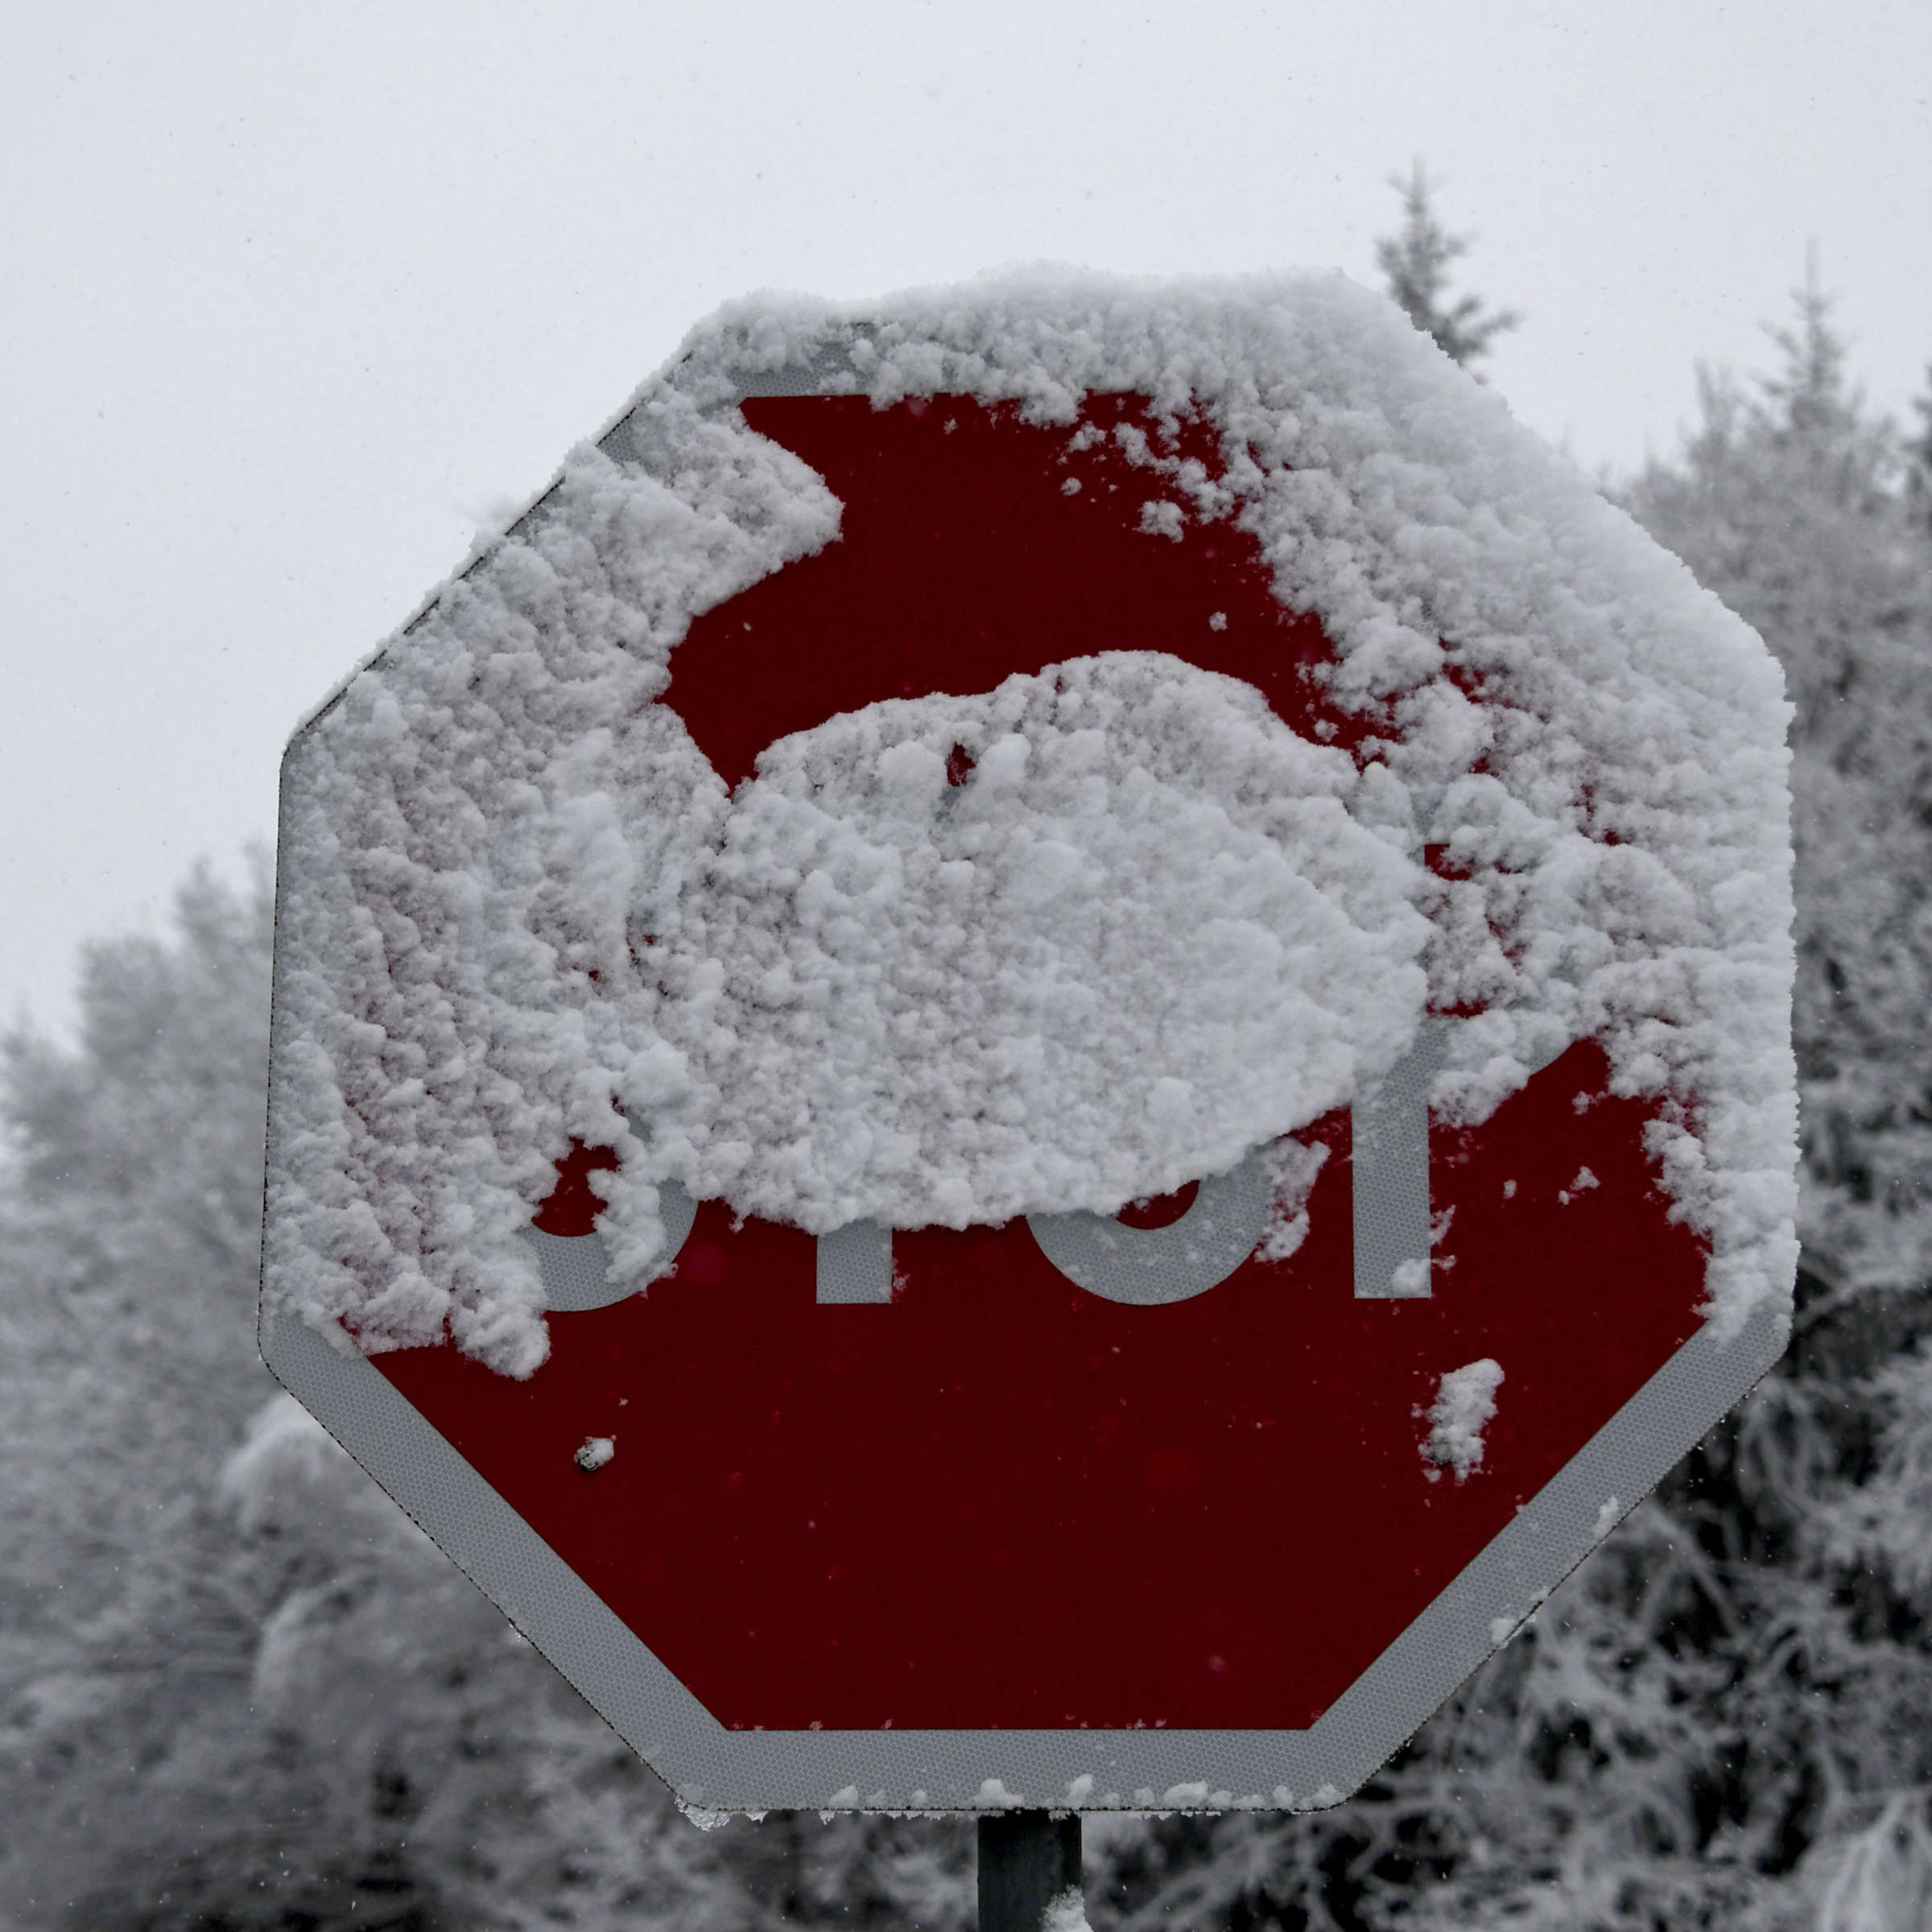
\includegraphics[height=\textwidth]{../images/Schilder Beispiele/Schnee.jpg}
       \caption{Witterung}
       \label{fig:witterung}
   \end{subfigure}
   \hspace{3em}%
   \begin{subfigure}[b]{0.125\textwidth}
       \centering
       
\includegraphics[height=\textwidth]{../images/Schilder Beispiele/MotionBlur.png}
       \caption{Unschärfe}
       \label{fig:motion-blur}
   \end{subfigure}
   \hspace{3em}%
   \begin{subfigure}[b]{0.125\textwidth}
       \centering
       \includegraphics[height=\textwidth]{../images/Schilder Beispiele/Überbelichtung}
       \caption{Belichtung}
       \label{fig:ueberbelichtung}
   \end{subfigure}
   \hspace{3em}%
   \begin{subfigure}[b]{0.125\textwidth}
    \centering
    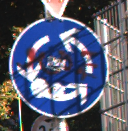
\includegraphics[height=\textwidth]{../images/Schilder Beispiele/Vandalismus.png}
    \caption{Vandalismus}
    \label{fig:vandalism}
   \end{subfigure}
      \caption{Weitere mögliche Einflüsse auf die Straßenschilderkennung}
      \label{fig:einfluesse-strscherkennung2}
\end{figure}

Ausgehend der Erkentnisse der Tests aus dem genannten Artikel, kann in einigen solcher Situationen davon ausgegangen werden, dass sich in vielen Fahrzeugen nicht auf die automatische Erkennung der Schilder verlassen werden kann. Ein Ziel der Hersteller ist das Anbieten von Fahrzeugen, die vollständig autonom, das heißt ohne menschliches Eingreifen, fahren können. Damit dies möglich ist, muss die Software der Fahrzeuge auch solche Grenzfälle korrekt interpretieren. Dies erfordert eine gewisse Menge an Daten, durch die diese Algorithmen trainiert werden.

Ziel dieser Arbeit ist ausgehend davon, gezielt Trainingsbilder erzeugen zu können, die einige dieser Aspekte simulieren. Es soll als alternative Möglichkeit dazu vorgeschlagen werden, sämtliche Trainingsdaten für Grenzfälle eigenständig in realen Fahrsituationen aufzunehmen.

%Diese EU-Verordnung verfolgt im wesentlichen das Ziel, verschiedene sicherheitsrelevante Systeme verpflichtend %einzuführen. Dazu zählen zudem Notbremsassistenten, Müdigkeitswarner und Notbremslichter. Die %Straßenschilderkennung trägt dazu im wesentlichen durch die Möglichkeit einer Warnung bei überhöhter %Geschwindgkeit oder einer automatischen Geschwindigkeitsanpassung bei.

\section{Künstliche Neuronale Netze}
\acused{KNN}
Durch künstliche neuronale Netze (\acsp{KNN}) können Maschinen lernen, bestimmte Probleme zu lösen, ohne dass ein Mensch vorher explizite Regeln dafür definieren muss. Dies steht im Kontrast zur Methode, der Maschine  vorher einen festen, vollständigen Regelsatz bereitzustellen. Letztgenannter Ansatz zeigt in einigen Gebieten nur begrenzten Erfolg, da es für Menschen herausfordernd sein kann, Regelsätze für Vorgänge zu definieren, die unbewusst im Gehirn stattfinden oder viel Kontext erfordern. Zu nennen sind hierbei die visuelle Objekterkennung oder menschliche Sprache. Außerdem können neue, nicht in den Regeln beachtete Situationen dazu führen, dass die Maschine das Problem nicht mehr lösen kann. Die Grundidee hinter \acp{KNN} ist deshalb, dass sich die Maschine selber einen Wissensschatz aufbaut, der ihr beim Lösen des Problems hilft. Dies geschieht, indem die Entwickler ihr reale Trainingsbeispiele zeigen. Möchte man einen Algorithmus trainieren, der Schach spielen soll, kann man ihm beispielsweise eine Vielzahl an realen Schachpartien zeigen. Anhand dessen lernt der Algorithmus verschiedene Strategien und baut ein Spielverständnis auf, das womöglich über die menschlichen Fähigkeiten hinausgeht. \cite[S. 1ff.]{DeepLearningBook}

In den letzten Jahrzehnten erlebte das maschinelle Lernen und damit auch das Gebiet der \acp{KNN} einen Aufschwung. Es existiert bereits seit Mitte des vergangenen Jarhunderts, wird allerdings erst durch die zunehmende Rechenleistung und die Verfügbarkeit von großen Datenmengen flächendeckend eingesetzt. Einsatzgebiete für \acp{KNN} sind unter anderem die Objekterkennung, das Verstehen von natürlicher Sprache und die Generierung von Text und Bildern. \cite[S. 4,17]{knnsKompakt}

Die Inspiration für \acp{KNN} bildet die Informationsverarbeitung des Gehirns in Lebewesen. Die kleinste hier betrachtete Einheit ist das Neuron. Neuronen in \acp{KNN} sind konzeptionell inspiriert von realen, biologischen Neuronen, besitzen aber eine deutlich abstrahierte Funktionsweise. In \acp{KNN} berechnen sie ein Skalarprodukt ihrer gewichteten Eingangswerte, addieren einen sogennaten \emph{Bias} hinzu und wenden auf das Ergebnis eine nichtlineare Funktion an. Letzere wird auch als Aktivierungsfunktion bezeichnet. Diese Aktivierungsfunktion kann analog dazu gesehen werden, dass biologische Neuronen einen Schwellenwert (\emph{engl.: threshold}) besitzen, der überschritten werden muss, damit das Neuron \emph{feuert}, also einen Impuls an weitere Neuronen weitergibt. Aktivierungsfunktionen sind notwendig, damit neuronale Netze Probleme lösen können, die über die Fähigkeiten einer linearen Regression hinausgehen. Es wird eine nichtlineare Abhängigkeit zwischen dem Eingang $X$ und dem Ausgang $Y$ umgesetzt. \cite{visualApproach}

In der Nachfolgenden Abbildung ist ein einzelnes künstliches Neuron eines \acp{KNN} darstellt. Das \emph{Plus-Zeichen} steht für die Berechnung des Skalarprodukts der Eingänge und der darauf addierte Bias. Die Aktivierungsfunktion wird durch das \emph{Sigmoid}-Zeichen simbolisiert. Der Ausgang (\emph{rechts}) ist das Ergebnis der Berechnung des Neurons. \cite{visualApproach}

\begin{figure}[H]
   \centering
   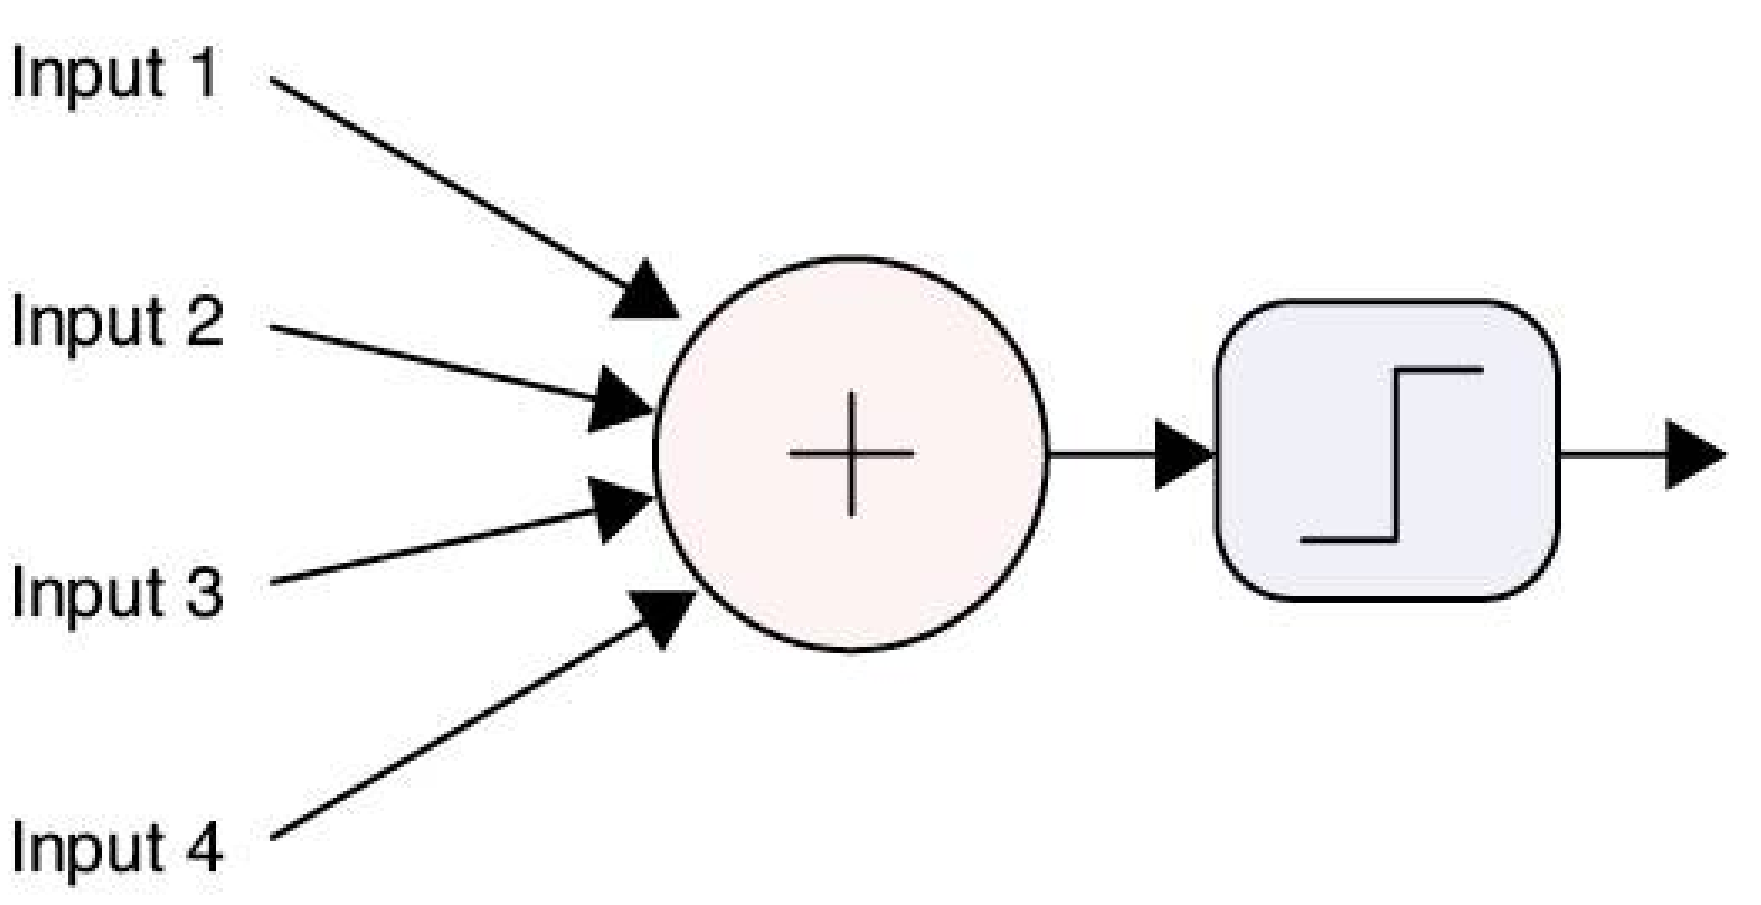
\includegraphics[width=0.5\textwidth]{images/KNNs/Neuron.png}
   \caption{Einzelnes Neuron eines \acp{KNN} \cite{visualApproach}}
\end{figure}

Um komplexe Probleme lösen zu können, werden mehre Neuronen miteinander verbunden und in Schichten angeordnet. Jede Schicht erhält die Ausgangswerte der vorherigen Schicht als Eingang und gibt die daraus berechneten, neuen Werte an die nächste Schicht weiter. In der nachfolgenden Abbildung sind die Neuronen durch Kreise dargestellt und ihre Verbindungen durch Linien. Eine Verbindung stellt dar, dass ein Neuron seinen berechneten Wert an das nachfolgende Neuron weitergibt. Dies geschieht hierbei ausschließlich von \emph{links nach rechts}, womit das \ac{KNN} als \emph{Feedforward-Netzwerk} bezeichnet wird. Die Eingabeschicht erhält die Eingabewerte des Netzwerks, die Ausgabeschicht liefert die Vorhersage des Modells. Zwischen diesen beiden Schichten befinden sich beliebig viele verarbeitende Schichten, die als \emph{Hidden Layer} bezeichnet werden. \cite{knnsKompakt}

\begin{figure}[H]
   \centering
   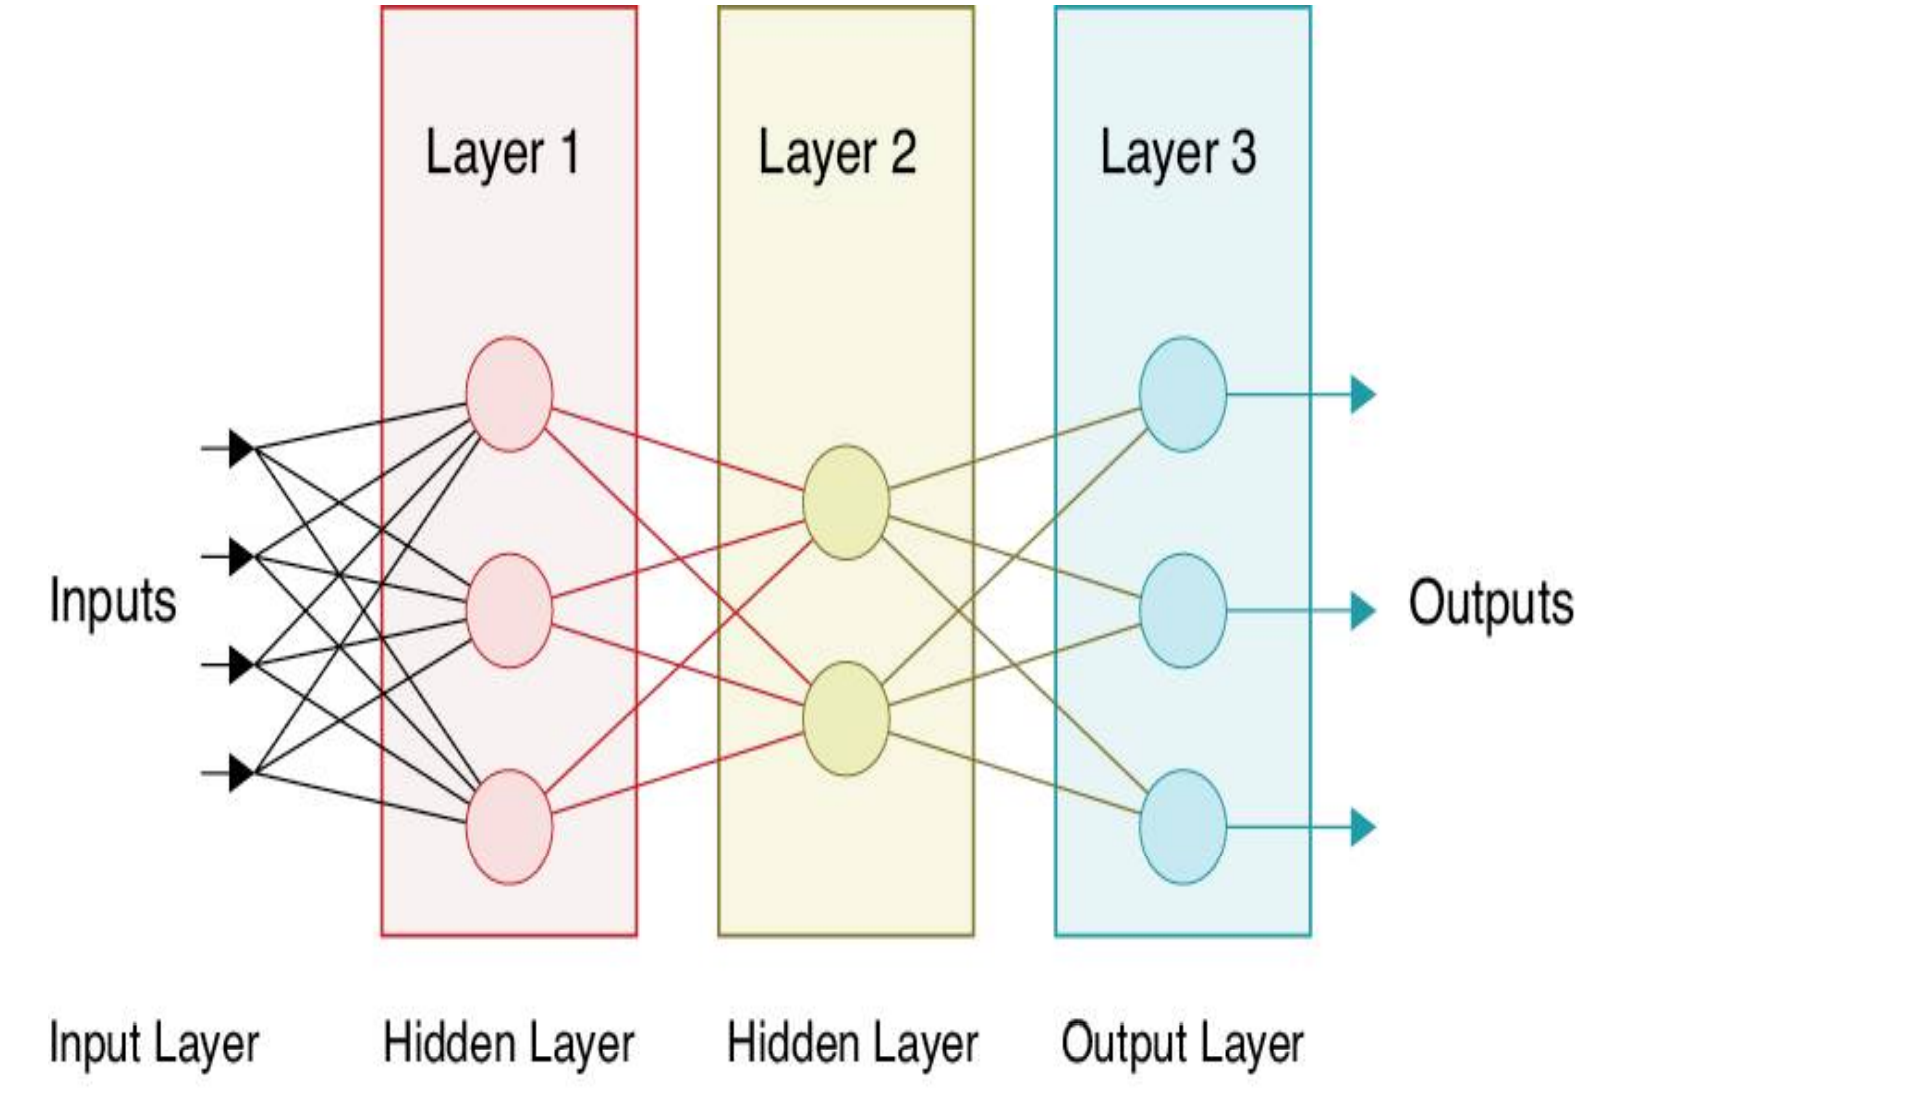
\includegraphics[width=0.7\textwidth]{images/KNNs/KNN_layers.png}
   \caption{Vollständiges \ac{KNN} \cite{visualApproach}}
\end{figure}

Die Vorhersage, gekennzeichnet durch die Werte der Ausgabeschicht, hängt von den jeweiligen Parametern der Neuronen des Netzwerks ab. Dies sind die Gewichte (\emph{engl.: weights}) der Verbindungen zwischen den Neuronen sowie der Bias der Neuronen. Es existieren auch trainierbare Aktivierungsfunktionen, diese sind jedoch vergleichsweise unüblich. Entwickler sind für den Entwurf der Netzwerkarchitektur zuständig, die Parameter werden jedoch durch das Modell trainiert. Zu Beginn besitzt das Modell zufällige Parameter, wodurch es in der Regel nicht die gewünschte Abbildung zwischen Ein- und Ausgabe implementiert. Ein untrainierter Schachalgorithmus spielt demnach augenscheinlich willkürliche Züge. Ein untrainierter Katzenklassifikator besitzt keinen erkennbaren Wissensschatz darüber, welche Charakteristiken eine Katze optisch auszeichnen. Das Ziel des Trainings ist, dass die Parameter des Modells zunehmend gegen das Optimum konvergieren und so das Modell immer plausibler in seinen Vorhersagen wird.

%---------------------------------------------------------------------------------------------------------------
\subsection{Training}
Damit ein neuronales Netz trainiert werden kann, bedarf es einer Funktion, die die Qualität der Vorhersagen des Modells bestimmt. Erst dadurch kann verglichen werden, ob eine gegebene Änderung der Parameter eine Annäherung an das globale Optimum zurfolge hat. Diese Funktion wird als \emph{Kostenfunktion} bezeichnet. Sie berechnet, gemittelt über alle $m$ Trainingsbeispiele $i$, die Abweichung des vorhergesagten Wertes $\hat{y}$ von dem tatsächlichen Wert $y$.
Die Kostenfunktion in Abhängigkeit von der Gesamtheit der Gewichte und Biases $\theta$ kann beispielsweise folgendermaßen definiert sein:
\begin{equation}
   \label{eq:costFunction}
   J(\theta) = \frac{1}{2m} \sum_{i=1}^{m} (\hat{y}^{(i)} - y^{(i)})^2
\end{equation}

Anstelle des Terms $\frac{1}{2}(\hat{y}^{(i)} - y^{(i)})^2$ können auch andere Metriken verwendet werden. Bezeichnet man dies verallgemeinert als Verlustfunktion $L$ \emph{(engl.: loss-function)}, so kann die Kostenfunktion wie folgt definiert werden:
\begin{equation}
   \label{eq:costFunctionGeneral}
   J(\theta) = \frac{1}{m} \sum_{i=1}^{m} L(\hat{y}^{(i)}, y^{(i)})
\end{equation}

Dies wird als überwachtes Lernen bezeichnet, da für die Berechnung der Kostenfunktion \emph{gelabelte} Trainingsdaten erforderlich sind. Das bedeutet, dass jedes Trainingsbild die zu erwartende Ausgabe enthält. Bei Bildern für einen Katzenklassifikator muss beispielsweise für jedes Trainingsbild durch einen Menschen gekennzeichnet werden, ob es eine Katze enthält oder nicht. Erst so kann bewertet werden, inwieweit die jeweiligen Vorhersagen des Modells korrekt sind.

Es ist jedoch nicht nur erforderlich, die Qualität der Vorhersagen des Netzes zu bestimmen. Um die Vorhersagen in zukünftigen Iterationen zu verbessern, ist es notwendig, die Parameter des Modells zu verändern. Darunter fallen, wie bereits erwähnt, die Gewichte und Biases $\theta$. Von ihnen hängt der Wert der Kostenfunktion ab. Die Ausgangssituation ist hierbei folgende: Mit einem gegebenen $\theta$ befindet man sich in einem bestimmten Punkt der Kostenfunktion $J(\theta)$. Gesucht ist eine Parameteränderung $\dif\theta$, mit der man sich am weitesten an das globale Minimum der Kostenfunktion annähert. Das globale Minimum ist die beste Lösung, die das Modell für die gegebenen Trainingsdaten finden kann und damit das Optimum.

Nähern tut man sich dem Optimum, indem man den Punkt $\theta$ in Richtung des negativen Gradienten der Kostenfunktion bewegt. Also die Richtung, in die, aus der momentanen Ausgangsposition, die Kostenfunktion den steilsten Abstieg besitzt. Pro Trainingsiteration nähert man sich dem Optimum nur um einen kleinen Betrag. Diese Annäherung wird als Gradientenabstieg bezeichnet, während der Betrag der Annäherung durch eine sogennante Lernrate $\alpha$ bestimmt wird. Die Lernrate ist ein \emph{Hyperparameter}, und damit klassischerweise ein nicht-trainierbarer Parameter, da sie durch die Entwickler fest bestimmt wird und nicht durch das Modell selbst gelernt wird. Es sind viele Trainingsschritte erforderlich, damit sich das Modell dem Optimum möglichst weit nähert. Der Gradientenabstieg muss demnach häufig durchgeführt werden.

Anhand der nachfolgenden Abbildung, soll der Gradientenabtieg visuell verdeutlicht werden.
%---------------------------------------------------------------------------------------------------------------
\subsection{Convolutional Neural Networks}
\acp{KNN} bewähren sich mitunter besonders im Bereich \emph{Computer Vision}. Ein Bereich, der sich mit der Interpretation von Bild- und Videodaten beschäftigt. Hier spielt die Mustererkennung eine tragende Rolle. Es sollen Merkmale erkannt werden, die jedes Objekt eines bestimmten Typs auszeichnen, die jedoch nicht auf jedem Bild die exakt identischen Pixelwerte besitzen. Die typische Form von Katzenohren ist beispielsweise ein Muster, das bei der Katzenerkennung verwendet werden kann. Es ist nicht trivial, allgemeine Regeln zu definieren, welche Pixelmuster als Katzenohr erkannt werden sollen und welche nicht. Deshalb wird hier auf \acp{KNN} zurückgegriffen.

Verwendet man hierfür jedoch die bisher beschriebene Netzwerkarchitektur, treten verschiedene Probleme auf. Jedes sogenannte \emph{Feature} des Eingangs wird über die Eingangsschicht in das \ac{KNN} gespeist. Bei einem Schachalgorithmus kann die Menge aller Features beispielsweise durch die momentane Position aller Figuren auf dem Schachbrett beschrieben werden. Das liegt daran, dass genau diese Werte den Ausgang des Netzwerks beeinflussen. In diesem Fall, welchen Zug der Algorithmus als nächstes spielt. Bei der Bildklassifizierung ist jeder Pixel des Bildes ein Feature. Ein Netz, das Bilder der Größe 1024x1024 Pixel klassifizieren soll, muss demnach folgende Anzahl an Eingängen verarbeiten:

\begin{equation}
   1024 \cdot 1024 = 1.048.576
\end{equation}

Um eine derartige Anzahl an Eingängen sinnvoll interpretieren zu können, ist ein Netzwerk mit vielen Schichten und Neuronen notwendig. So vielen, dass auch heutige Computer an die grenzen ihrer Rechenleistung gelangen. Mitunter deshalb wird im Bereich Computer Vision auf \acp{CNN} zurückgegriffen. Der Begriff \emph{Convolution}, zu deutsch \emph{Faltung}, gibt einen Hinweis auf die Funktionsweise dieser Netze. Schichten, die so eine Faltung in einem \ac{CNN} durchführen, werden als \emph{Convolutional Layers} bezeichnet.



\section{Bildgenerierung mittels Künstlicher Neuronaler Netze}
\label{chap:NoGANs}

Der Lernfortschritt von Klassifikatoren besteht darin, besser in der Aussage zu werden, ob ein Label $y$ auf einen gegebenen Eingang $x$ zutrifft. Dafür benötigen sie annotierte Trainingsdaten. Schachalgorithmen sollen hingegen lernen, Züge zu spielen, die die Gewinnchancen des Algorithmus maximieren. Eine weitere Art von \acp{KNN} sind \emph{generative Netze}. Sie sollen lernen, neue Daten zu erzeugen, die der Verteilung der Trainingsdaten ähneln. Generative Netze zur Bildgenerierung sollen demnach anhand eines Trainingsdatensatzes lernen, welche Bilder sie erzeugen sollen. Dies lernen sie anhand der statistischen Verteilung der Trainingsdaten. Die Daten sind nicht annotiert, wodurch generative Netze in der Regel in das \emph{Unüberwachte Lernen} einzuordnen sind.

\subsection{Mathematischer Hintergrund}
Generative Netze zur Bilderzeugung sollen beurteilen können, wie wahrscheinlich es ist, dass ein gegebenes Bild aus der Verteilung der Trainingsdaten stammt. Wenn $x$ für jedes mögliche existierende Bild steht, so bilden generative Netze folgende Wahrscheinlichkeitsverteilung ab:
\begin{equation}
   \hat{p}(x)
\end{equation}
Für ein gegebenes Bild $x$ gibt $\hat{p}(x)$ einen Schätzwert dafür an, wie wahrscheinlich es ist, dass das Bild aus den Trainingsdaten stammt. Diese Wahrscheinlichkeitsverteilung wird durch das Netz erlernt. Optimiert wird, dass die geschätzte Verteilung der Daten $\hat{p}(x)$ möglichst ähnlich zu der tatsächlichen Verteilung der Trainingsdaten $p(x)$ ist. Ein beispielhafter Vergleich ist in Abbildung \ref{fig:generativeNetsPx} dargestellt. Es ist erkennbar, dass sich die geschätzte und die tatsächliche Verteilung ähnlich sehen, jedoch nicht identisch sind. Die Abweichung zwischen diesen Verteilungen stellt dabei die Kosten (engl.: den \emph{loss}) dar. Die schwarzen Punkte kennzeichnen Trainingsdaten. Durch sie soll die Verteilung $p(x)$ abgebildet werden. Weniger diversifizierte Trainingsdaten würden sich beispielsweise nur in einem Teilbereich von $p(x)$ befinden. Dadurch könnte das Modell $p(x)$ weniger gut approximieren.

\begin{figure}[H]
   \centering
   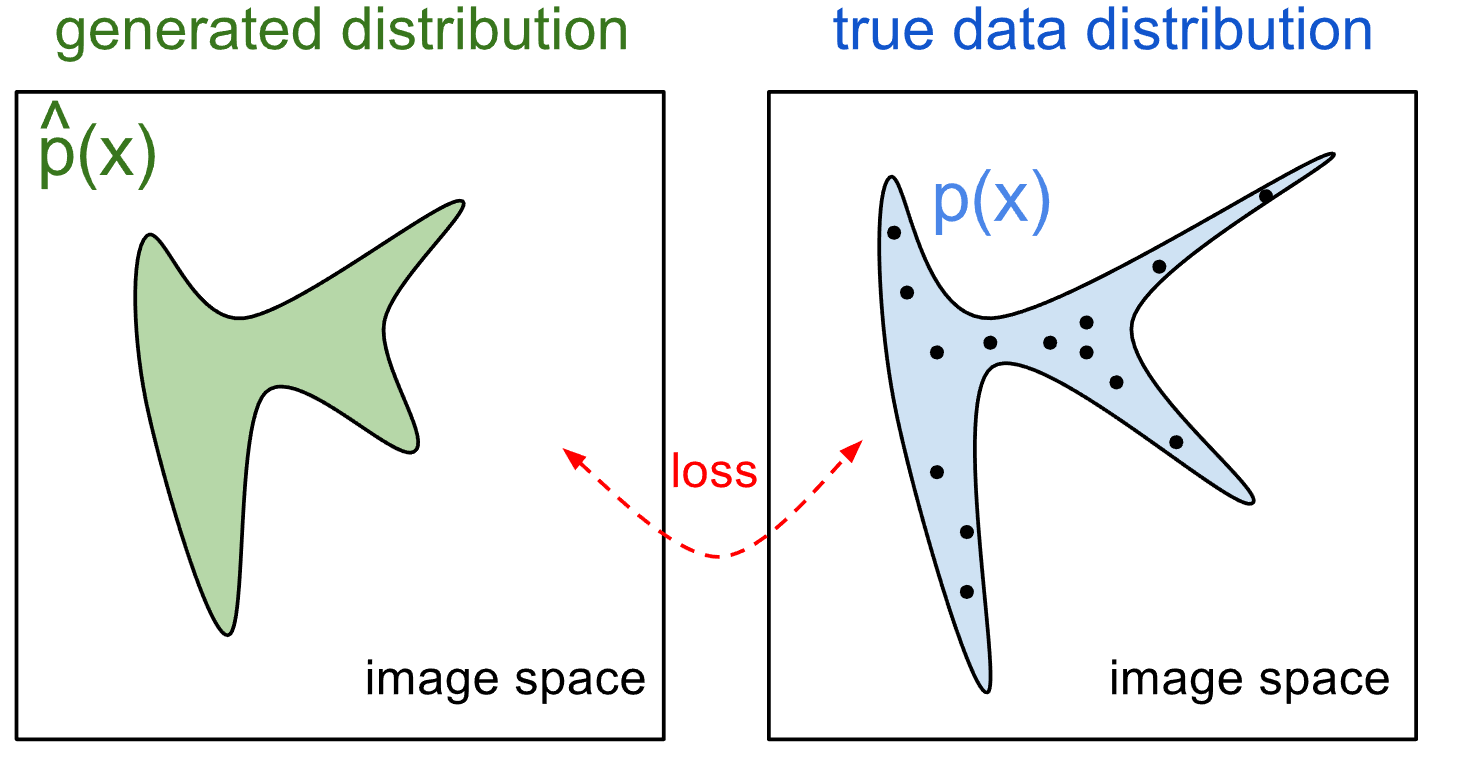
\includegraphics[width=0.5\textwidth]{images/Generative Networks/p(x) Distribution.png}
   \caption{Beispielhafter Vergleich von $\hat{p}(x)$ und $p(x)$ \cite{openAiGenerativeNets}}
   \label{fig:generativeNetsPx}
\end{figure}

Bei der Bildgenerierung versucht das Netz den Wahrscheinlichkeitswert für $\hat{p}(x)$ zu maximieren. Es erlernt durch $\hat{p}(x)$, wie die Verteilung der Trainingsdaten aussieht und versucht anschließend ausschließlich Bilder zu generieren, die dieser Verteilung folgen. Bezogen auf Abbildung \ref{fig:generativeNetsPx} befinden sich alle generierten Bilder des trainierten Netzes im grün markierten Bereich.

Es existieren verschiedene Arten generativer Netze. Die Taxonomie, also die Einteilung verschiedener Netze in bestimmte Kategorien, kann Abbildung \ref{fig:generativeModelsTaxonomy} entnommen werden. Einerseits existieren Architekturen, die die Wahrscheinlichkeitsverteilung $\hat{p}(x)$ explizit berechnen. Andere berechnen die Funktion nicht, verwenden sie jedoch implizit. In der Abbildung wird dahingehend zwischen \emph{Explicit Density Models} \emph{(explizit berechnete Dichte)} und \emph{Implicit Density Models} \emph{(implizit berechnete Dichte)} unterschieden. Es existieren zudem Unterkategorien, mittels derer eine feinere Kategorisierung durchgeführt wird.

\begin{figure}[H]
   \centering
   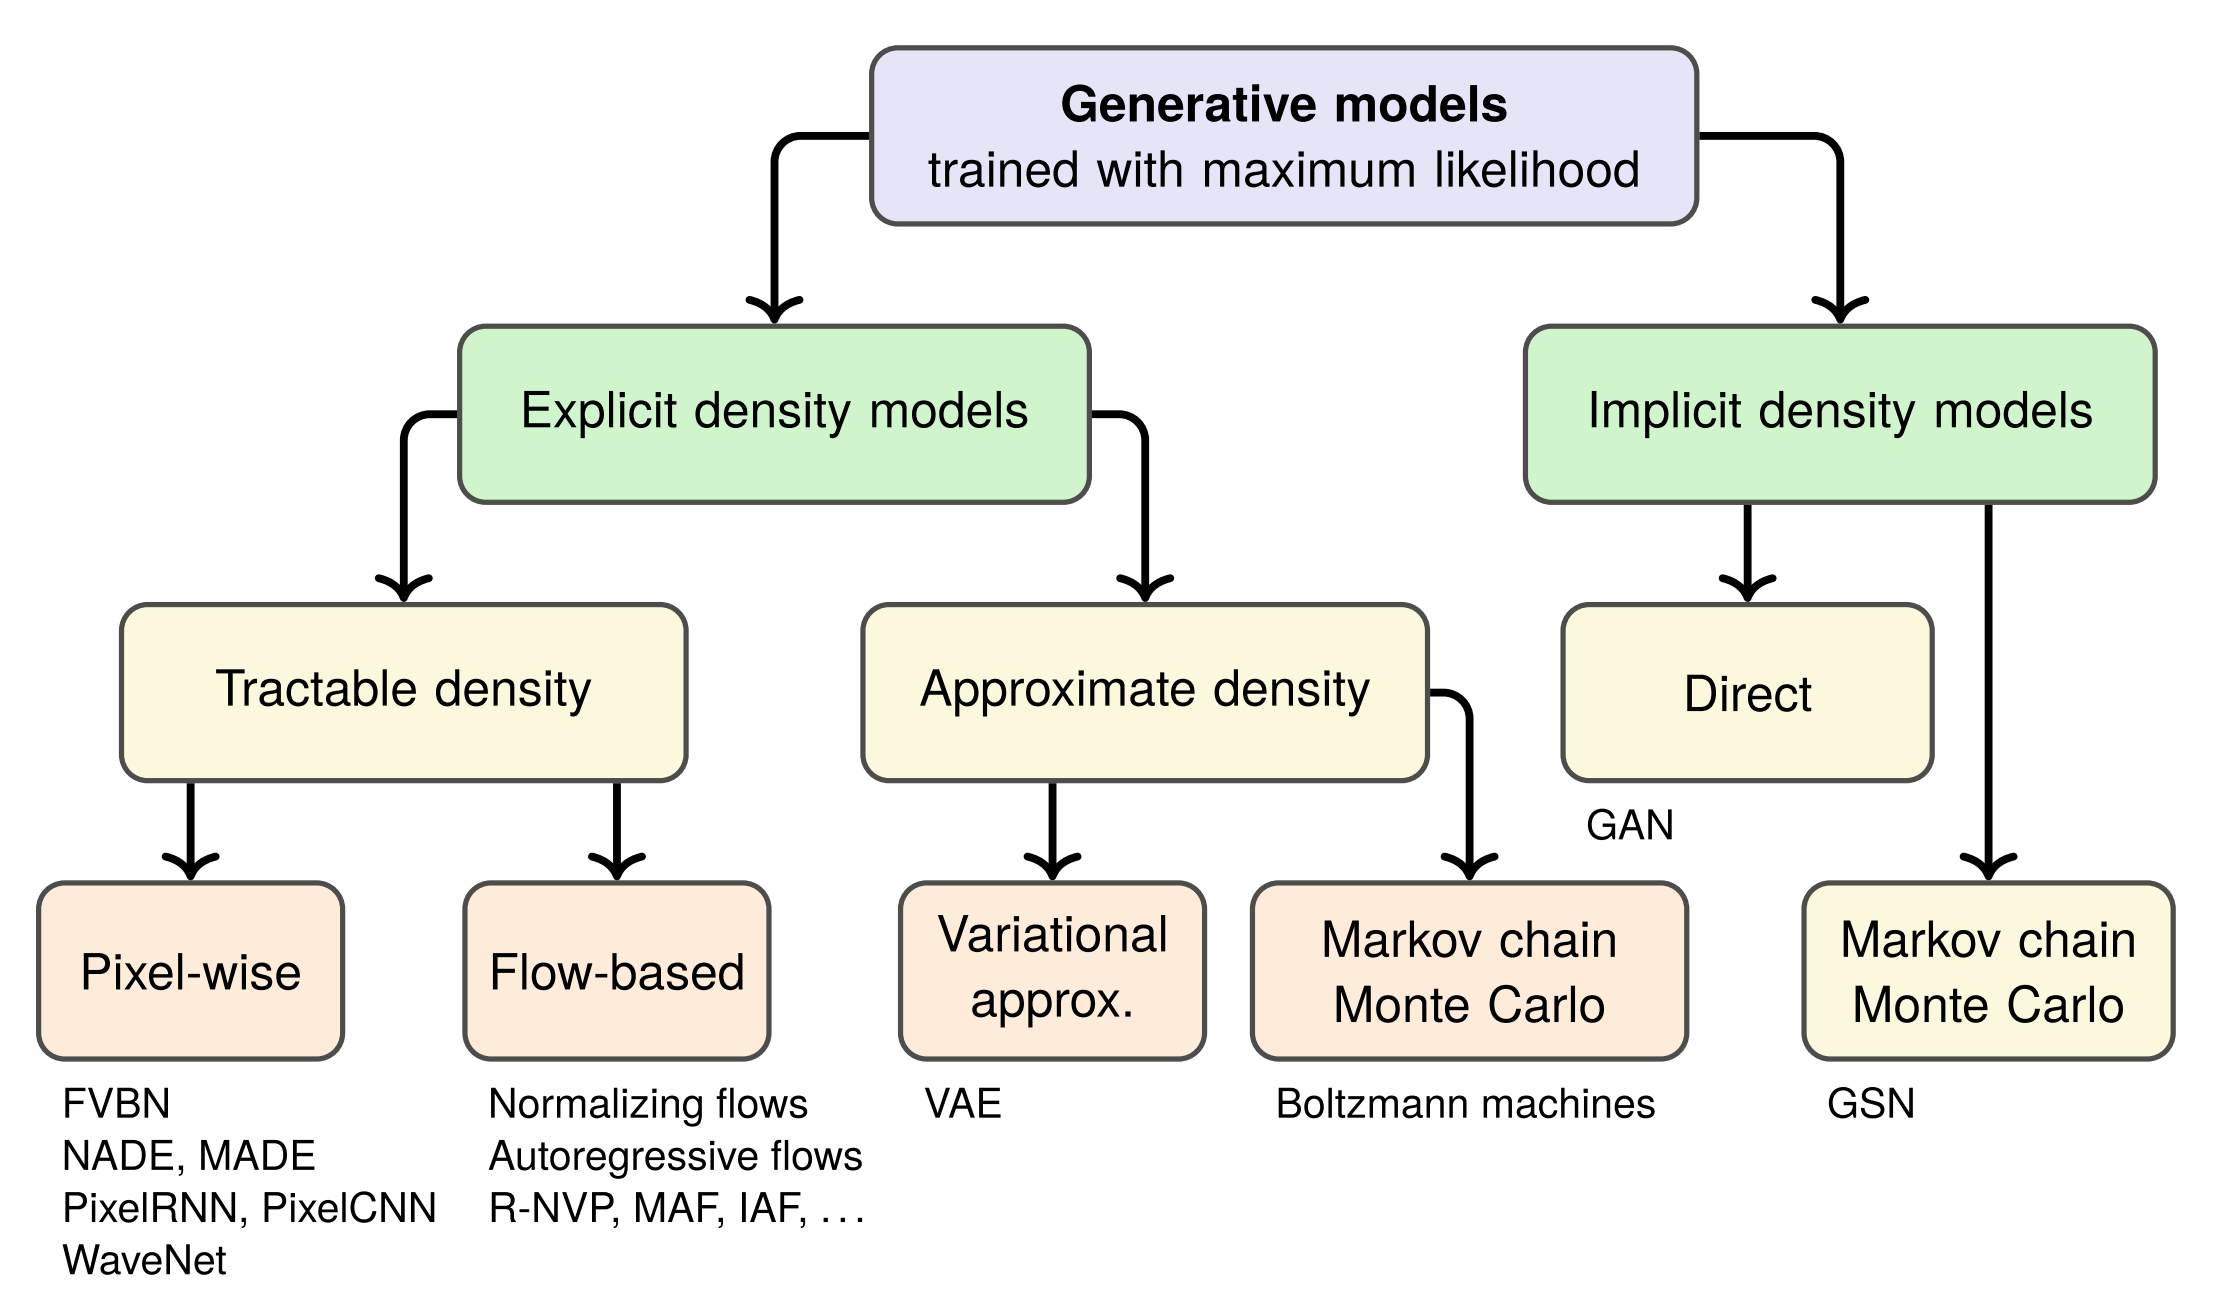
\includegraphics[width=0.8\textwidth]{images/Generative Networks/Taxonomy of Generative Models.png}
   \caption{Taxonomie generativer Modelle \cite{generativeModelsBook}}
   \label{fig:generativeModelsTaxonomy}
\end{figure}

Es soll in diesem Kapitel auf verschiene Architekturen generativer Netze eingegangen werden. \acp{GAN} werden gesondert in Kapitel \ref{chap:GANs} beschrieben.

\subsection{Pixel Recurrent Neural Networks}
Die Architektur der \acp{PixelRNN} stammt aus dem Jahr 2016. Diese Netze stützen sich explizit auf die Maximierung der Maximum-Likelihood-Schätzung von $\hat{p}(x)$ für jeden Pixel. Sie sind in der genannten Taxonomie den Modellen zuzuordnen, die den tatsächlichen Schätzwert von $p(x)$ berechnen können. \cite{pixelRNN}

Im folgenden soll geklärt werden, wie der optimale Wert für jeden Pixel eines generierten Bildes bestimmt wird. Ein betrachtetes Bild $x$ der Auflösung $n \times n$ kann in seine einzelnen Pixel $(x_{1}, x_{2}, ..., x_{n^2})$ aufgeteilt werden. In Gleichung \ref{eq-max-likelihood} ist dabei dargestellt, wie die Wahrscheinlichkeit eines jeden Pixels in die gesamte Verteilung $\hat{p}(x)$ einfließt. \cite{pixelRNN}
\begin{equation}
   \label{eq-max-likelihood}
   \hat{p}(x) = \hat{p}(x_{1}, x_{2}, ..., x_{n^2}) = \prod_{i=1}^{n^2}\hat{p}(x_{i}|x_{1},...,x_{i-1})
\end{equation}
Jeder Pixel $x_{i}$ besitzt eine eigene Wahrscheinlichkeitsverteilung $\hat{p}(x_{i}|x_{1},...,x_{i-1})$. Sie ist abhängig von allen anderen Pixeln $x_{1},...,x_{i-1}$ des Bildes. Der absolut optimale Wert eines Pixels kann demnach nur dann berechnet werden, wenn die Werte aller anderen Pixel bekannt sind. Das Produkt aller Wahrscheinlichkeitswerte der einzelnen Pixel ergibt $\hat{p}(x)$. Soll $\hat{p}(x)$ maximiert werden, so müssen die Terme $\hat{p}(x_{i}|x_{1},...,x_{i-1})$ möglichst hohe Werte liefern. Daraus ergibt sich dann unter gegebenem Kontext für jeden Pixel eine Maximum-Likelihood-Schätzung. Also der Wert, für den $\hat{p}(x)$ möglichst weit gegen \emph{eins} strebt. \cite{pixelRNN}

Die Idee von PixelRNNs ist, dass bei der Generierung in einer Ecke des Bildes gestartet wird. Das Bild wird zunächst auf einen Pixel reduziert, der im folgenden $x_{1}$ genannt wird. Für diesen Pixel wird ein Wert generiert. Anschließend wird $x_{1}$ gemeinsam mit einem benachbarten Pixel $x_{2}$ betrachtet. Die Wahrscheinlichkeitsverteilung für $x_{2}$ ergibt sich dadurch zu $\hat{p}(x_{2}|x_{1})$. Der Wert für $x_2$ ist somit nur von $x_1$ abhängig. Da $x_{1}$ bekannt ist, kann ein optimaler Wert für $x_{2}$ bestimmt werden. Die Wahrscheinlichkeitsverteilung von $x_{3}$ ergibt sich zu $\hat{p}(x_{3}|x_{1}, x_{2})$, die von $x_{4}$ zu $\hat{p}(x_{4}|x_{1}, x_{2}, x_{3})$. Das Bild wird sukzessive generiert, wobei der momentane Pixelwert für $x_{i}$ von allen bisher generierten Pixeln abhängig ist. Dieses vorgehen ist in Abbildung \ref{fig:pixelRNN} dargestellt. Der Wert des rot markierten Pixels hängt von allen blau markierten Pixel ab. Ist für diesen ein Wert bestimmt, wird der rechtsseitig benachbarte Pixel als neues $x_{i}$ gewählt.

\begin{figure}[H]
   \centering
   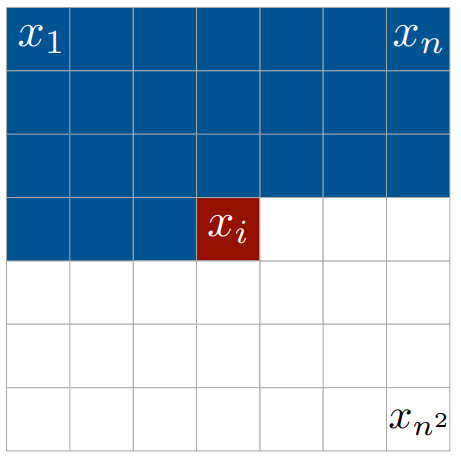
\includegraphics[width=0.25\textwidth]{images/Generative Networks/PixelRNN.png}
   \caption{Bestimmung von $\hat{p}(x)$ mit PixelRNNs \cite{pixelRNN}}
   \label{fig:pixelRNN}
\end{figure}

Um die beschriebene Abhängigkeit des momentan generierten Pixels zu allen bisher generierten Pixel umsetzen zu können, besitzen \acp{PixelRNN} eine Art \emph{Erinnerung}. Bisher wurden in dieser Arbeit nur sogenannte \emph{Feedforward} Netze behandelt, bei denen der Informationsfluss stets in eine Richtung erfolgt. Nämlich vom Eingang des Netzes zum Ausgang. Es existieren auch \emph{Recurrent Neural Networks}. Sie werden besonders zur Verarbeitung von natürlicher Sprache eingesetzt \emph(engl.: natural language processing). Abbildung \ref{fig:RNN} bildet hierfür eine beispielhafte Darstellung.

\begin{figure}[H]
   \centering
   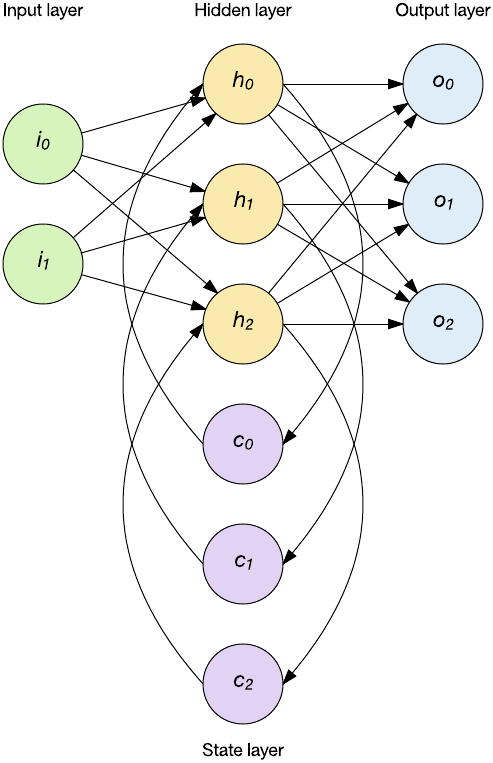
\includegraphics[width=0.375\textwidth]{images/Generative Networks/RNN.png}
   \caption{Darstellung eines Recurrent Neural Networks \cite{ibmRNN}}
   \label{fig:RNN}
\end{figure}

In Recurrent Neural Networks spielen die \emph{Zustände} eines Netzes eine besondere Rolle. Ein Zustand wird durch die Eingangs- und Ausgangswerte aller Neuronen zu einem gegebenen Zeitpunkt beschrieben. In \acp{PixelRNN} ist der Zustand des Netzes für den Pixel $x_{2}$ abhängig von dem Zustand des Netzes für $x_{1}$. Um solche Beziehungen darstellen zu können, besitzt das beispielhaft abgebildete Netz die Neuronen $c_{0}$ bis $c_{2}$, die den vorherigen Wert eines Neurons rekursiv auf seinen Eingang zurückführen. Somit wird der vorherige Zustand des neuronalen Netzes als zusätzlicher Eingang für die Berechnungen genutzt. \acp{PixelRNN} nutzen eine besondere Form der Recurrent Neural Networks. Sie arbeiten mit sogenannter \emph{Long Short-term Memory}. Dadurch soll das Problem behoben werden, dass in klassischen Recurrent Neural Networks weit in der Vergangenheit liegende Zustände nur noch einen geringen Einfluss auf den momentanen Zustand haben. \cite{generativeModelsSurvey}

Da die durch ein \ac{PixelRNN} umgesetzte Verteilung $\hat{p}(x)$ direkt erfassbar ist, wird ihnen nachgesagt, dass die Performanz solcher Netze gut evaluiert werden kann. Es gilt als vergleichsweise leicht, für solche Netze Metriken zur Messung der Performanz umzusetzen. Ein grundlegender Nachteil von \acp{PixelRNN} ist, dass die Generierung sequenziell erfolgt. Es ist in dem beschriebenen Verfahren nicht möglich, mehrere Pixel parallel zu generieren, da der Wert eines Pixels von denen aller vorher generierten Pixel abhängig ist. Dies verlangsamt die Generierung, da keine Parallelisierung möglich ist. \cite{generativeModelsSurvey}

Es existieren auch sogenannte \emph{PixelCNNs}, bei denen sich die Berechnung stets nur auf bestimmte Bildbereiche konzentriert. Diese Bildbereiche können parallel zueinander sequenziell berechnet werden. Die Parallelisierung ist jedoch nur während des Trainings des Netzwerks oder während der Evaluation von $\hat{p}(x)$ für gegebene Bilder möglich. Die Bildgenerierung erfolgt auch hier, analog zu \acp{PixelRNN}, vollständig sequenziell. \cite{pixelRNN}

\subsection{Autoencoder}

Das Ziel von Autoencodern ist, den Eingang des Netzes am Ausgang zu rekonstruieren. Dazu setzen sich diese Netze aus drei Bestandteilen zusammen: dem Kodierer, dem latenten Raum und dem Dekodierer. In Abbildung \ref{fig:Autoencoder} ist eine beispielhafte Autoencoderarchitektur dargestellt.

\begin{figure}[H]
   \centering
   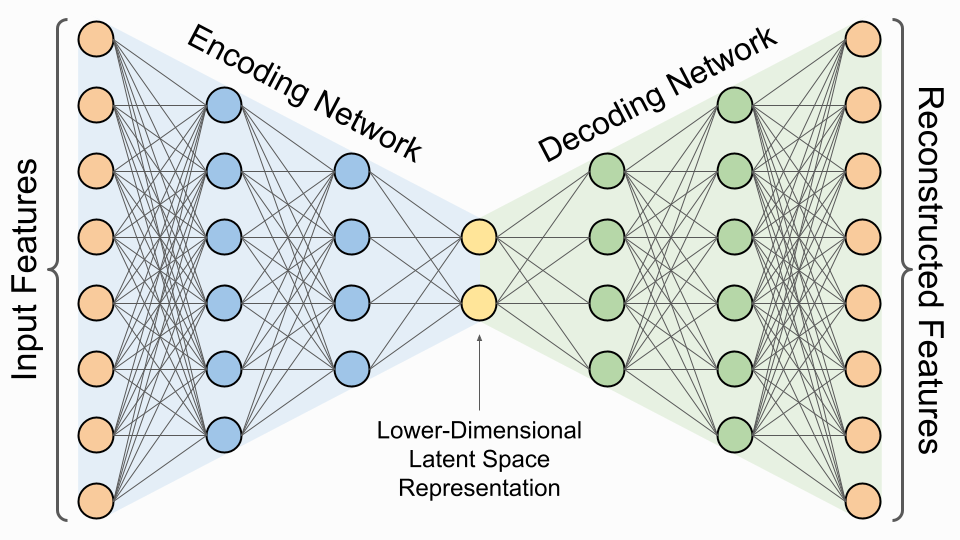
\includegraphics[width=0.65\textwidth]{images/Generative Networks/autoencoder_architecture.png}
   \caption{Architektur eines Autoencoders}
   \label{fig:Autoencoder}
\end{figure}

Der \textbf{Kodierer} besitzt die Aufgabe, Merkmale aus dem Eingang des Netzes zu extrahieren. Diese Merkmale sollen daraufhin mit einer begrenzten Anzahl an Parametern durch den latenten Raum repäsentiert werden. Somit besteht die Aufgabe des Kodierers darin, den Eingang auf seine für das Netz wesentlichen Eigenschaften zu reduzieren. Und zwar erfolgt die Komprimierung dabei so, dass die Informationen gerade so durch den latenten Raum dargestellt werden können. 

Bei dem \textbf{latenten Raum} handelt es sich um eine einzelne Schicht von Parametern, oder in diesem Kontext: Neuronen. Je mehr Neuronen sich in dem latenten Raum befinden, desto mehr Informationen können von der Kodierung an die Dekodierung übertragen werden. Die Merkmale, die sich in dem latenden Raum befinden, können durch einen Vektor $\vec{z}$ beschrieben werden. Der latente Raum sollte klein genug sein, damit dort nicht alle Merkmale des Eingangs gespeichert werden können. So wird der Kodierer dazu gezwungen, vereinzeilte Merkmale zu extrahieren. 

Der \textbf{Dekodierer} nutzt die Werte aus dem latenten Raum, um den Eingang nachzubilden. Diese Nachbildung stellt den Ausgang des Autoencoders dar. Die Kosten eines Autoencoders können durch die Abweichung zwischen Ein- und Ausgang festgestellt werden. 

Da der Zweck von Autoencodern darin besteht, einen Eingang auf seine relevanten Merkmale zu reduzieren, wird der Dekodierer nur während des Trainings verwendet. Beim praktischen Einsatz eines Autoencoders werden lediglich der Kodierer und der latente Raum eingesetzt. Im Gegensatz zu \acp{PixelRNN} basieren Autoencoder klassischerweise nicht auf Recurrent Neural Networks, sondern auf Feedforward Netzen.

Diese beschriebene Architektur der Autoencoder ist nicht für die generative Modellierung geeignet, da sie deterministisch ist. Erhält das Modell bestimmte Eingangswerte, so liefert es stets die gleichen Ausgangswerte. Es versucht den Eingang möglichst zu rekonstruieren, wobei der Inhalt $\vec{z}$ des latenten Raums für ein gegebenes Eingangsbild stets gleich ist. Eine zufällige Erzeugung neuer Bilder ist damit nicht möglich. Die sogenannten \emph{Variational Autoencoder} sind eine Architektur, die für die Generierung neuer Daten verwendet werden können. \cite{visualApproach}

\textbf{Variational Autoencoder} verfolgen das Ziel, eine Zufallskomponente in die Bilderzeugung einfließen zu lassen. Ein entscheidender Unterschied zu klassischen Autoencodern ist deshalb der folgende: Ein gegebener Eingang $x$ wird auf kein festes $\vec{z}$ kodiert, sondern auf eine Wahrscheinlichkeitsverteilung. Sie wird bezeichnet als:
\begin{equation}
   p(z|x)
\end{equation}
Im Gegensatz zu \acp{PixelRNN} versucht das Netz somit nicht die Verteilung der Trainingsdaten $p(x)$ zu approximieren, sondern die Verteilung der Merkmale $\vec{z}$ der Trainingsdaten $x$.
Es wird angenommen, dass jedes Merkmal normalverteilt ist. Damit kann jede Komponente $z_{i}$ des Vektors $\vec{z} = [z_{1}, z_{2}, ..., z_{n}]^\mathsf{T}$ durch eine Gaußsche Normalverteilung $\mathcal{N}(\mu_{i}, {\sigma_{i}}^{2})$ beschrieben werden. Aufgabe des Kodierers ist damit nicht mehr, aus einem gegebenen $x$ eine Menge von Merkmalen $\vec{z}$ zu bestimmen. Stattdessen soll der Kodierer die Vektoren $\vec{\mu}$ und $\vec{\sigma}$ bestimmen, durch die sich die einzelnen Normalerteilungen von $\vec{z}$ beschreiben lassen. 

An den Dekodierer wird ein zufällig aus der Verteilung $p(z|x)$ entnommenes Set an Merkmalen $\vec{z}$ übergeben.
Der Dekodierer übersetzt dieses gegebene $\vec{z}$ daraufhin in ein Bild. Im praktischen Einsatz werden bei einem Variational Autoencoder nur der latente Raum und der Dekodierer genutzt. Der Dekodierer erhält zufällige Werte für $\vec{z}$, also zufällige Merkmale, und generiert daraus ein Bild.

\textbf{Vor- Nachteile?}

\cite{autoencoders}

\label{chap:GANs}
\subsection{Generative Adversarial Networks}
Eine weitere Architektur, die zur Bildgenerierung verwendet werden kann, sind die sogenannten \emph{Generative Adversarial Networks} (\acsp{GAN}). Sie wurden unter anderem von Ian Goodfellow im Jahre 2014 entwickelt.

Ein \ac{GAN} besteht aus zwei Komponenten. Dem \emph{Generator} und dem \emph{Discriminator}.
Der Generator erzeugt aus einem zufälligen Eingangsvektor ein Bild. Der Discriminator erhält ein Bild als Eingang und gibt entweder den Wert \emph{0} oder den Wert \emph{1} aus. Er soll erkennen, ob das gegebene Bild aus den Trainingsdaten stammt, oder ob es künstlich generiert wurde. Bei sowohl dem Generator als auch dem Discriminator handelt es sich um \acp{KNN}. Diese beiden Komponenten werden so miteinander gekoppelt, dass der Discriminator stets entweder ein erzeugtes Bild des Generators oder ein Bild aus den Trainingsdaten erhält. Dies ist in der nachfolgenden Abbildung beispielhaft dargestellt:
\begin{figure}[H]
	\centering
	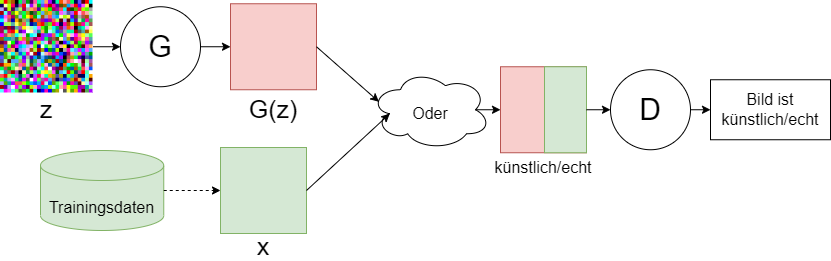
\includegraphics[width=0.8\textwidth]{../images/GANs/GAN.drawio.png}
	\caption{Zusammenspiel zwischen Generator und Discriminator}
	\label{fig:gan}
\end{figure}
Der Generator G erhält einen zufälligen Eingangsvektor $z$. Letzterer kann als ein weißes Rauschen beschrieben werden. Das generierte Bild ist das Resultat der Funktion $G(z)$ des Generators G. Anschließend wird dem Discriminator D entweder das generierte Bild $G(z)$ oder ein Bild $x$ aus den Trainingsdaten gezeigt. Der Ausganswert des Discriminators ist daraufhin die Einschätzung, ob das gezeigte Bild echt oder künstlich generiert ist. Ziel des Generators ist, dass die Verteilung der künstlichen Daten $p(G(z))$ möglichst ähnlich der Verteilung $p(x)$ ist. Der Discriminator soll die beiden Verteilungen möglichst gut voneinander unterscheiden können. Somit handelt es sich um ein direktes Gegenspiel zwischen Generator und Discriminator. Sie versuchen sich gegenseitig zu überlisten.

\paragraph{Training}
Dies spiegelt sich auch im Training von \acp{GAN} wider. $V(D,G)$ stellt die zu optimierende Funktion dar: \cite{Goodfellow-GANs}
\begin{equation}
   \label{eq:adv_loss}
	\min_{G} \max_{D} V(D,G) = \mathbb{E}_{x}[\log(D(x))] + \mathbb{E}_{z}[\log(1-D(G(z)))]
\end{equation}
Bei dem Training handelt es sich um ein Min-Max-Problem. Der Generator versucht die Funktion $V(G,D)$ zu minimieren, wohingegen der Discriminator sie zu maximieren versucht. Der Term \ref{eq:real_adv_loss} stellt die Fehlerrate des Discriminators auf den echten Trainingsdaten dar. Mit anderen Worten: Wie viele echte Bilder er als unecht klassifiziert. Der Term \ref{eq:fake_adv_loss} beschreibt, wie viele unechte Daten der Discriminator als echt klassifiziert. \cite{visualApproach}
\begin{equation}
   \label{eq:real_adv_loss}
	\mathbb{E}_{x}[\log(D(x))]
\end{equation}
\begin{equation}
   \label{eq:fake_adv_loss}
	\mathbb{E}_{z}[\log(1-D(G(z)))]
\end{equation}
Der Term \ref{eq:real_adv_loss} ist nicht vom Generator abhängig, sondern lediglich von $D(x)$. Hierauf hat der Generator keinen Einfluss, wodurch er alleine durch diesen Teil der Kostenfunktion nicht trainiert wird. Der Discriminator besitzt somit zwei Terme, die ihn trainieren, während der Generator nur einen besitzt. Aus diesem Grund werden dem Discriminator in der Regel doppelt so viele unechte Daten wie echte Trainingsdaten gezeigt. Dies soll einem ungleichen Training der beiden Komponenten des \acp{GAN} entgegenwirken. Der Optimalzustand eines \acp{GAN} ist, dass der Discriminator so gut wie möglich identifizieren kann, ob ein gegebenes Bild aus $p(x)$ stammt, während der Generator dennoch in der Lage ist, den Discriminator zu überlisten. Das Training von \acp{GAN} gilt als empfindlich gegenüber den gewählten Hyperparametern und der Netzwerkarchitektur. \acp{GAN} wird nachgesagt, dass kleine Änderungen in den beiden genannten Aspekten die Qualität der Generierten Bildern signifikant beeinflussen können. \cite{visualApproach}

Im praktischen Einsatz wird nur der Generator des \acp{GAN} verwendet. Der Discriminator wird ausschließlich dazu eingesetzt, mit $p(G(z))$ möglichst gut $p(x)$ zu approximieren, sodass die generierten Bilder im Optimalfall nicht von echten Trainingsdaten zu unterscheiden sind. \cite{visualApproach}
%Analog zu Kapitel \ref{chap:NoGANs}, ist die Aufgabe des Generators, Daten aus der Wahrscheinlichkeitsverteilung $p(x)$ der Trainingsdaten zu erzeugen. Der Eingangsvektor $z$ des Generators folgt einer Verteilung $p_z(z)$. Der Generator kann durch folgende Funktion beschrieben werden:

%\begin{equation}
%	G(z, \theta_{g})
%\end{equation}

%Der Generator erzeugt neue Bilder, während der Discriminator für jedes erzeugte Bild rät, ob es aus dem Trainingssatz stammt, oder ob es künstlich generiert ist. Nur der Discriminator hat dabei Zugriff auf den Trainingsdatensatz. Ihm werden klassischerweise abwechselnd Bilder aus dem Trainingssatz und erzeugte Bilder des Generators gezeigt. Die beiden Komponenten des \acp{GAN} agieren dabei stets gegeinander. Der Generator versucht den Discriminator in die Irre zu führen, dass seine generierten Bilder in Wahrheit aus dem Trainingssatz stammen würden, während der Discriminator versucht, möglichst gut zu erkennen, ob ein Bild echt ist oder nicht. Bei beiden Komponenten handelt es sich dabei um künstliche neuronale Netze \acused{KNN}(\acp{KNN}). \cite{visualApproach}

%\subsection{Spieltheorie}
%Aus spieltheoreticher Sicht kann das Gegenspiel von Generator und Discriminator auch als \emph{Nullsummenspiel} %betrachtet werden.
%Zu Beginn werden sowohl der Generator als auch der Discriminator mit zufälligen Parametern initialisiert. Dadurch ist zu erwarten, dass 


%Der Generator erzeugt Bilder, die denen des Trainingssatzes nicht änhlich sind, während der Discriminator noch nicht weiß, was die Bilder des Trainingssatzes einzigartig macht. Durch das Training verbessern sich beide Komponenten in ihren Aufgaben. Sie trainieren sich gegenseitig, da sie beide versuchen, das Spiel zu gewinnen.

%Das finale Optimum ist, dass der Discriminator so gut in der Unterscheidung zwischen echten und künstlichen Daten wird, wie mit den vorhandenen Daten nur möglich, während der Generator trotzdem in der Lage sein soll, den Discriminator zu überlisten. \cite[S. 656]{visualApproach}

%Während die Bildklassifizierung ein Minimierungsproblem ist, stellt die Bildgenerierung mittels \acp{GAN} ein Min-Max-Problem dar. Bei ersterem wird versucht, die Loss-Function zu minimieren, sodass die Predictions möglichst gut den Labels der Daten entsprechen. Bei \acp{GAN} besteht der Unterschied darin, dass einerseits der Generator die Loss-Function zu minimieren versucht, während andererseits der Discriminator sie zu maximieren versucht.

%\begin{equation}
%	\min_{G} \max_{D} V(D,G) = \mathbb{E}_{x}[\log(D(x))] + \mathbb{E}_{z}[\log(1-D(G(z)))]
%\end{equation}
Die bisher beschriebene Architektur von \acp{GAN} wird auch als \emph{Vanilla \ac{GAN}} bezeichnet. Dies entspricht dem, wie \acp{GAN} in Goodfellows Publikation definiert werden \cite{Goodfellow-GANs}. Forscher und Anwender haben seit dieser Veröffentlichung verschiedene Limitationen und Probleme bei Vanilla \acp{GAN} feststellen können. Insbesondere im Hinblick auf spezielle Einsatzgebiete. Ein hier häufig anzutreffender Begriff ist \emph{Modal Collaps}. Damit ist die Situation gemeint, dass der Generator bei beliebigem Input stets dasselbe Bild generiert. Er lernt, dass ein bestimmtes Bild den Discriminator überlisten kann und generiert es deshalb jedes Mal, egal welchen Input man ihm zuführt. Dies ist für diesen Anwendungsfall insofern von Relevanz, alsdass der Generator verschiedene Arten von Straßenschildern generieren soll, wobei jedes Bild zusätzlich einen unterschiedlichen Hintergrund besitzen soll. Lösen lässt sich das Problem des \emph{Modal Collaps} beispielsweise mit sogenannten \acp{CycleGAN}. \cite{visualApproach}

\paragraph{CycleGANs}
Ein \ac{CycleGAN} besteht aus zwei miteinander gekoppelten \acp{GAN}. Diese werden klassischerweise als $G$ und $F$ bezeichnet. Bei $G$ handelt es sich um ein Vanilla \ac{GAN}, so wie in diesem Kapitel bisher beschrieben. Erweitert wird das Netzwerk jedoch so, dass es den Output von $G$ an $F$ weitergibt. $F$ erhält somit das von $G$ künstlich generierte Bild als Input. Aufgabe von $F$ ist, daraus den ursprünglichen Input, der $G$ zugeführt wurde, zu reproduzieren. Somit soll das gesamte Netzwerk nicht nur neue Bilder generieren können, sondern soll auch von einem generierten Bild zurück auf den zugeführten Input schließen können. Dies lässt sich mathematisch so darstellen, dass $G$ und $F$ folgende Abbildungen implementieren:
\begin{equation}
	\mathbf{G}: X\mapsto Y \: \wedge \: \mathbf{F}: Y\mapsto \tilde{X}
\end{equation}
Das Modell $G$ erzeugt somit aus einem gegebenen $X$ ein $Y$, wohingegen $F$ aus dem $Y$ auf das $X$ schließen soll. Die Behebung des Modal Collaps findet dadurch statt, dass das Netzwerk den Output $\tilde{X}$ von $F$ überprüft und diesen mit dem tatsächlichen Input $X$ vergleicht. Es wird überprüft, wie ähnlich sich $\tilde{X}$ und $X$ sind. Liegt eine zu hohe Diskrepanz vor, kann das Netzwerk darauf schließen, dass $G$ Outputs erzeugt, die nicht in direkter Abhängigkeit zu $X$ stehen.

\acp{CycleGAN} sind für spezielle Anwendungsgebiete gedacht, in denen ausgewählte, und somit nicht-zufällige Eingabewerte verwendet werden. Dazu zählen Gebiete wie \emph{Style Transfer} oder die Transformation von Bildern, respektive Bildelementen. Diese Studienarbeit stellt eine solche Problemstellung dar, da das auf dem generierten Bild gezeigte Straßenschild durch den Eingang des Netzwerks definiert wird.

Das Training von \acp{CycleGAN} basiert auf mehreren Kostenfunktionen. Die \acp{GAN} $G$ und $F$ besitzen jeweils einen eigenen \emph{Adversarial Loss}. Damit ist die in Gleichung \ref{eq:adv_loss} beschriebene Kostenfunktion eines Vanilla \acp{GAN} gemeint. Im Kontext von \acp{CycleGAN} ist sie, für das \ac{GAN} G wie folgt definiert:
\begin{equation}
	L_{GAN}(G, D_Y, X, Y) = \mathbb{E}_y[\log{D_Y(y)}] + \mathbb{E}_x[\log(1-D_Y(G(x)))]
\end{equation}
Die Funktion für \ac{GAN} F ist identisch, mit dem Unterschied, dass sie von $F$ und $D_X$ statt von $G$ und $D_Y$ abhängt.

Als weitere Kostenfunktion besitzen \acp{CycleGAN} einen \emph{Cyclic Loss} (Gleichung \ref{eq:cycle-loss}). Die beiden Summanten der Gleichung setzen sich daraus zusammen, wie weit die Pixelwerte von den generierten Bildern und den echten Bildern auseinander liegen. Mit $G(x)$ wird ein Bild $\tilde{y}$ generiert, $F$ generiert anschließend aus diesem $\tilde{y}$ wieder ein $\tilde{x}$. Wenn $\tilde{x}$ und $x$ möglichst ähnlich sind, dann kann davon ausgegangen werden, dass die generierten Bilder des Netzwerks $G$ in direkter Abhängigkeit von dem Input $X$ stehen. Was hierbei berechnet wird, ist die durschnittliche, absolute Abweichung der Pixelwerte.
\begin{equation}
   \label{eq:cycle-loss}
	L_{cyc}(G, F) = \mathbb{E}_x[||F(G(x))-x||_1] + \mathbb{E}_y[||G(F(y))-y||_1]
\end{equation}
Um die gesamten Kosten des \acp{CycleGAN} zu erhalten, werden die bisher beschriebenen Kostenfunktionen addiert. Der \emph{Cyclic Loss} $L_{cyc}(G, F)$ wird dabei mit einem absoluten Wert $\lambda$ multipliziert, um die Kosten dieser Funktion im Vergleich zu den \emph{Adversarial Losses} gewichten zu können. In der Veröffentlichung der \acp{CycleGAN} wird ein $\lambda$ von $10$ verwendet. Somit wird mit einem vergleichweise hohen Gewicht versehen, dass die generierten Bilder in direkter Abhängigkeit zu den Eingangswerten des \acp{CycleGAN} stehen. Der Wert $\lambda$ stellt einen Hyperparamer dar. \cite{cycleGAN}
\begin{equation}
	L(G, F, D_X, D_Y) = L_{GAN}(G, D_Y, X, Y) + L_{GAN}(F, D_X, Y, X) + \lambda \cdot L_{cyc}(G, F)
\end{equation}
\cite{cycleGAN}

\paragraph{Wasserstein GANs}
\textbf{Auf Taxonomie eingehen}

%In dieser Studienarbeit sollen \acp{GAN} zur Generierung künstlicher Bilder von Straßenschildern eingesetzt %werden. Dies ist jedoch nicht die einzige Möglichkeit, wie mittels \acp{KNN} künstliche Bilder erzeugt werden %können. In diesem Kapitel werden daher weitere Methoden vorgestellt, die ebenfalls dazu eingesetzt werden können.

%Eines der bisher genannten Beispiele für \acp{KNN} ist die Umsetzung eines Katzenklassifikators. Diese sogenannten %diskriminativen Modelle setzen grundlegend folgende Wahrscheinlichkeitsfunktion um:
%\begin{equation}
%   p(y|x)
%\end{equation}
%Bei einem Eingang $x$ soll das Modell die Wahscheinlichkeit für jeden Ausgang $y$ bestimmen. Zeigt man einem %Katzenklassifikator ein Bild auf dem keine Katze zu sehen ist, so soll $p(\mathrm{Katze}|x)$ gering sein. Die %Wahrscheinlichkeiten einer Wahrscheinlichkeitsverteilung müssen zusammen den Wert \emph{eins} ergeben, wodurch im %Umkehrschluss der Ausgang $p(\mathrm{KeineKatze}|x)$ eine hohe Wahrscheinlichkeit liefert. Um diese Verteilung %erlernen zu können, ist Supervised Learning notwendig.

%Generative Netze besitzen eine andere Aufgabe. Sie sollen neue Verteilungen generieren. Diese Verteilungen sollen %möglichst ähnlich der Verteilung sein, auf die das Modell trainiert wurde. Das Modell bestimmt, wie wahrscheinlich %es ist, dass ein gegebenes $x$ aus der Verteilung stammt. Konkret bezogen auf den Kontext dieser Studienarbeit: %Gibt man dem generativen Modell ein Bild, soll es bestimmen, wie wahrscheinlich es ist, dass dies ein real %aufgenommenes Foto eines Straßenschildes ist. Es wird folgende Wahrscheinlichkeitsfunktion umgesetzt:
%\begin{equation}
%   p(x)
%\end{equation}
%Wobei $p(x)$ als die Wahrscheinlichkeit interpretiert werden kann, dass ein gegebenes $x$ aus der Verteilung der %Trainingsdaten stammt.

%\subsection{Boltzmann Maschinen}
%\subsection{Deep Belief Netzwerke}

%\section{Generative Adversarial Networks}
%\acp{GAN} sind eine der eingesetzten Methoden, um Algorithmen zu entwickeln, die neue Daten künstlich generieren können. Dazu zählen zum Beispiel Bilder von Menschen, die zwar realistisch erscheinen, die so aber in der Realität nicht existieren. Die Aufgabe eines \acp{GAN} ist demnach, Daten zu generieren, die denen des definierten Trainingssatzes in einer solchen Weise ähneln, dass nicht mehr unterschieden werden kann, ob ein Bild künstlich generiert ist oder aus dem Trainingssatz stammt. In dem genannten Beispiel besteht der Trainingssatz aus echten Bildern von Menschen, durch die das \ac{GAN} lernt, neue Bilder zu erzeugen. Im weiteren Verlauf wird das Thema \acp{GAN} ausschließlich auf die Bilderzeugung bezogen, auch wenn ebenso andere Anwendungsgebiete existieren. \cite{visualApproach}

Ein \ac{GAN} besteht aus zwei Komponenten. Dem sogenannten \emph{Generator} und dem \emph{Discriminator}. Der Generator erzeugt neue Bilder, während der Discriminator für jedes erzeugte Bild rät, ob es aus dem Trainingssatz stammt, oder ob es künstlich generiert ist. Nur der Discriminator hat dabei Zugriff auf den Trainingsdatensatz. Ihm werden klassischerweise abwechselnd Bilder aus dem Trainingssatz und erzeugte Bilder des Generators gezeigt. Die beiden Komponenten des \acp{GAN} agieren dabei stets gegeinander. Der Generator versucht den Discriminator in die Irre zu führen, dass seine generierten Bilder in Wahrheit aus dem Trainingssatz stammen würden, während der Discriminator versucht, möglichst gut zu erkennen, ob ein Bild echt ist oder nicht. Bei beiden Komponenten handelt es sich dabei um künstliche neuronale Netze \acused{KNN}(\acp{KNN}). \cite{visualApproach}

Während die Bildklassifizierung ein Minimierungsproblem ist, stellt die Bildgenerierung mittels \acp{GAN} ein Min-Max-Problem dar. Bei ersterem wird versucht, die Loss-Function zu minimieren, sodass die Predictions möglichst gut den Labels der Daten entsprechen. Bei \acp{GAN} besteht der Unterschied darin, dass einerseits der Generator die Loss-Function zu minimieren versucht, während andererseits der Discriminator sie zu maximieren versucht.

\begin{equation}
	\min_{G} \max_{D} V(D,G) = E_x[\log(D(x))] + E_z[\log(1-D(G(z)))]
\end{equation}

\subsection{Spieltheorie}
Aus spieltheoreticher Sicht kann das Gegenspiel von Generator und Discriminator auch als \emph{Nullsummenspiel} betrachtet werden.

\subsection{Training}
Zu Beginn sind sowohl der Generator als auch der Discriminator nicht gut geeignet für ihre jeweiligen Aufgaben. Der Generator erzeugt Bilder, die denen des Trainingssatzes nicht änhlich sind, während der Discriminator noch nicht weiß, was die Bilder des Trainingssatzes einzigartig macht. Durch das Training verbessern sich beide Komponenten in ihren Aufgaben. Sie trainieren sich gegenseitig, da sie beide versuchen, das Spiel zu gewinnen.

Das finale Optimum ist, dass der Discriminator so gut in der Unterscheidung zwischen echten und künstlichen Daten wird, wie mit den vorhandenen Daten nur möglich, während der Generator trotzdem in der Lage sein soll, den Discriminator zu überlisten. \cite[S. 656]{visualApproach}

\textbf{Bild ist nicht 100\% korrekt! G wird z.B. nicht trainiert, wenn D richtig lag, aber das Bild aus dem Datensatz stammte.}
\begin{figure}[H]
	\centering
	\includegraphics[width=\linewidth]{../images/GAN-Prozess.drawio.pdf}
	\caption{Trainingsprozess von GANs (angelehnt an \cite[S. 654f.]{visualApproach})}
	\label{fig:gan-trainingsprozess}
\end{figure}

(Auf Emfindlichkeit von GANs für Hyperparameter eingehen)

\subsection{Architekturen}
Die bisher beschriebene Architektur von \acp{GAN} wird auch als \emph{Vanilla \ac{GAN}} bezeichnet. Dies entspricht dem, wie \acp{GAN} in Goodfellows Publikation definiert werden \cite{Goodfellow-GANs}. Forscher und Anwender haben seit dieser Veröffentlichung verschiedene Limitationen und Probleme bei Vanilla \acp{GAN} feststellen können. Insbesondere im Hinblick auf spezielle Einsatzgebiete. Ein hier häufig anzutreffender Begriff ist \emph{Modal Collaps}. Damit ist die Situation gemeint, dass der Generator bei beliebigem Input stets dasselbe Bild generiert. Er lernt, dass ein bestimmtes Bild den Discriminator überlisten kann und generiert es deshalb jedes Mal, egal welchen Input man ihm zuführt. Lösen lässt sich dieses Problem beispielsweise mit sogenannten \acp{CycleGAN}.

\paragraph{CycleGANs}
Ein \ac{CycleGAN} besteht aus zwei miteinander gekoppelten \acp{GAN}. Diese werden klassischerweise als $G$ und $F$ bezeichnet. Bei $G$ handelt es sich um ein Vanilla \ac{GAN}, so wie in diesem Kapitel bisher beschrieben. Erweitert wird das Netzwerk jedoch so, dass es den Output von $G$ an $F$ weitergibt. $F$ erhält somit das von $G$ künstlich generierte Bild als Input. Aufgabe von $F$ ist, daraus den ursprünglichen Input, der $G$ zugeführt wurde, zu reproduzieren. Somit soll das gesamte Netzwerk nicht nur aus einem Input einen gewissen Output generieren können, sondern soll auch von einem gegebenen Output zurück auf den Input schließen können. Dies lässt sich mathematisch so darstellen, dass $G$ und $F$ folgende Abbildungen implementieren:
\begin{equation}
	\mathbf{G}: X\mapsto Y \: \wedge \: \mathbf{F}: Y\mapsto X
\end{equation}
Das Modell $G$ erzeugt somit aus einem gegebenen $X$ ein $Y$, wohingegen $F$ aus dem $Y$ auf das $X$ schließen soll. Die Behebung des Modal Collaps findet dadurch statt, dass das Netzwerk den Output $\tilde{X}$ von $F$ überprüft und diesen mit dem tatsächlichen Input $X$ vergleicht. Es wird überprüft, wie ähnlich sich $\tilde{X}$ und $X$ sind. Liegt eine zu hohe Diskrepanz vor, kann das Netzwerk darauf schließen, dass $G$ Outputs erzeugt, die nicht in direkter Abhängigkeit zu $X$ stehen. 

Was deutlich wird, ist dass hierbei die Idee verworfen werden muss, $G$ ein weißes Rauschen als Input zuzuführen. \acp{CycleGAN} sind für spezielle Anwendungsgebiete gedacht, in denen ausgewählte, und somit nicht-zufällige Eingabebilder verwendet werden. Dazu zählen Gebiete wie \emph{Style Transfer} oder die Transformation von Bildern, respektive Bildelementen. Es wird sich im Verlauf der Arbeit zeigen, dass die Problemstellung dieser Studienarbeit ein solches Anwendungsgebiet darstellt.

\begin{equation}
	L_{GAN}(G, D_Y, X, Y) = E_y[\log{D_Y(y)}] + E_x[\log(1-D_Y(G(x)))]
\end{equation}
\begin{equation}
	L_{cyc}(G, F) = E_x[||F(G(x))-x||_1] + E_y[||G(F(y))-y||_1]
\end{equation}
\begin{equation}
	L(G, F, D_X, D_Y) = L_{GAN}(G, D_Y, X, Y) + L_{GAN}(F, D_X, Y, X) + \lambda L_{cyc}(G, F)
\end{equation}
\cite{cycleGAN}
\paragraph{Wasserstein GANs}

\cite{DeepLearningBook}
\cite{visualApproach}

\section{Vorherige Arbeiten}
Durch eine Recherche haben sich zwei Arbeiten gezeigt, die sich, analog zu dieser Studienarbeit, mit der künstlichen generierung von Straßenschildern mittels \acp{KNN} beschäftigen. Beide Arbeiten konzentrieren sich darauf, Bildausschnitte zu erzeugen, die ein Straßenschild zeigen und eine geringfügige Menge an Hintergrund um das Schild.

\subsection{Generierung Taiwanischer Straßenschilder mittels DCGAN}
Eine der beiden Arbeiten wurde im Jahr 2021 veröffentlicht. Sie konzentriert sich auf die Generierung taiwanischer Straßenschilder. Dafür wird ein \emph{DCGAN} verwendet, ein \ac{GAN}, das im Generator und im Discriminator eine tiefe \ac{CNN} Architektur besitzt. Getestet wird, inwiefern künstlich generierte Trainingsbilder die Erkennung von Straßenschildern verbessern können. Es werden in der Arbeit vier Arten von Verkehrsschildern generiert. \cite{taiwanGAN}
%\begin{figure}[H]
%   \centering
%   \captionsetup[subfigure]{labelformat=empty}
%   \begin{subfigure}{0.075\textwidth}
%       \centering
%       \includegraphics[height=\textwidth]{../images/Taiwan Schilder/Taiwan_road_sign_禁-25.svg.png}
%       \phantomsubcaption
%   \end{subfigure}
%   \hspace{2em}%
%   \begin{subfigure}{0.075\textwidth}
%       \centering
%       \includegraphics[height=\textwidth]{../images/Taiwan Schilder/600px-Taiwan_road_sign_禁-1.svg.png}
%       \phantomsubcaption
%   \end{subfigure}
%   \hspace{2em}%
%   \begin{subfigure}{0.075\textwidth}
%       \centering
%       
\includegraphics[height=\textwidth]{../images/Taiwan Schilder/Taiwan_road_sign_r5-60.svg.png}
%       \phantomsubcaption
%   \end{subfigure}
%   \hspace{2em}%
%   \begin{subfigure}{0.075\textwidth}
%    \centering
%    \includegraphics[height=\textwidth]{../images/Taiwan Schilder/Taiwan_road_sign_禁-26.svg.png}
%    \phantomsubcaption
%   \end{subfigure}
%      \caption{Generierte Arten von taiwanischen Schildern \cite{taiwanGAN}}
%      \label{fig:taiwan-schilder}
%\end{figure}

Für jede der vier Klassen wird das \ac{GAN} mit 350 Bildern trainiert. Die Bildgrößen variieren dabei, wobei die Maximalgröße bei 200x200 Pixel liegt. Die generierten Bildgrößen korrespondieren zu denen der Trainingsbilder. Es sollen in der Arbeit bewusst keine größeren Bilder als 200x200 Pixel erzeugt werden, da Straßenschilder häufig nur einen kleinen Teil des Sichtfelds auf der Straße ausmachen.
Das Training erstreckt sich auf bis zu 2000 Epochen, was bedeutet, dass das \ac{GAN} während des Trainings 2000 mal alle Trainingsbilder als Eingabe erhält. \cite{taiwanGAN}

Da die Anzahl an Trainingsbildern beschränkt ist, generiert das Modell keine völlig neuartigen Bilder, sondern für jede Klasse jeweils vergleichsweise ähnlich aussehende:

\begin{figure}[H]
    \centering
    \captionsetup[subfigure]{labelformat=empty}
    \begin{subfigure}{0.125\textwidth}
        \centering
        
\includegraphics[height=\textwidth]{../images/Taiwan Schilder/Generated0.png}
        \phantomsubcaption
    \end{subfigure}
    \hspace{2em}%
    \begin{subfigure}{0.125\textwidth}
        \centering
        
\includegraphics[height=\textwidth]{../images/Taiwan Schilder/Generated1.png}
        \phantomsubcaption
    \end{subfigure}
    \hspace{2em}%
    \begin{subfigure}{0.125\textwidth}
        \centering
        
\includegraphics[height=\textwidth]{../images/Taiwan Schilder/Generated2.png}
        \phantomsubcaption
    \end{subfigure}
    \hspace{2em}%
    \begin{subfigure}{0.125\textwidth}
     \centering
     
\includegraphics[height=\textwidth]{../images/Taiwan Schilder/Generated3.png}
     \phantomsubcaption
    \end{subfigure}

    %\hspace{2em}%
    \begin{subfigure}{0.125\textwidth}
        \centering
        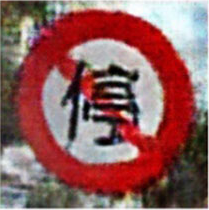
\includegraphics[height=\textwidth]{../images/Taiwan Schilder/Generated4.png}
        \phantomsubcaption
    \end{subfigure}
    \hspace{2em}%
    \begin{subfigure}{0.125\textwidth}
        \centering
        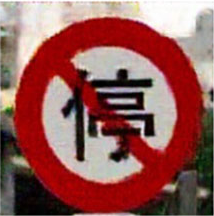
\includegraphics[height=\textwidth]{../images/Taiwan Schilder/Generated5.png}
        \phantomsubcaption
    \end{subfigure}
    \hspace{2em}%
    \begin{subfigure}{0.125\textwidth}
        \centering
        
\includegraphics[height=\textwidth]{../images/Taiwan Schilder/Generated6.png}
    \phantomsubcaption
    \end{subfigure}
    \hspace{2em}%
    \begin{subfigure}{0.125\textwidth}
        \centering
        
\includegraphics[height=\textwidth]{../images/Taiwan Schilder/Generated7.png}
    \phantomsubcaption
    \end{subfigure}
       \caption{Beispielergebnisse der Generierung taiwanischer SChilder \cite{taiwanGAN}}
       \label{fig:taiwan-gen-schilder}
 \end{figure}

Zur Beurteilung der Generierung wird mitunter der sogenannte \ac{SSIM} verwendet. Statt dass beispielsweise die Differenz aller entsprechenden Pixelwerte berechnet wird, werden hier die Aspekte \emph{Kontrast}, \emph{Leuchtdichte} und \emph{Struktur} der generierten und der echten Bilder verglichen. Dafür werden keine Berechnungen mit einzelnen Pixelwerten durchgeführt, sondern es wird mit den Mittelwerten und der Standardabweichung der Pixelwerte gerechnet. Auf die zugehörigen Formeln wird in Kapitel \ref{chap:Evaluation} eingegangen. \cite{taiwanGAN}

Der Nutzen der generierten Bildern wird anhand eines Modells zur Objektdetektion getestet. In dem Fall, ein sogenanntes \emph{YOLO} Modell. Die Detektion erfolgt auf größeren Bildern, auf denen mehrere Straßenschilder zu sehen sind. Für das Training des Modells werden mit etwa gleicher Gewichtung die für das \ac{GAN} verwendete Trainingsdaten und generierte Daten des \acp{GAN} verwendet. Zur Evaluation wurden hierbei Bilder verwendet, die insgesamt 40 Straßenschilder beinhalten. Die Ergebnisse können folgender Tabelle entnommen werden: \cite{taiwanGAN}

\begin{table}[H]
    \centering
    \begin{tabular}{|l||c|c||l|}
    \hline
    Modell   & \begin{tabular}[c]{@{}c@{}}Reale Trainingsbilder?\end{tabular} & \begin{tabular}[c]{@{}c@{}}Künstliche Trainingsbilder?\end{tabular} & \begin{tabular}[c]{@{}c@{}} Genauigkeit\end{tabular} \\ \hline \hline
    Densenet & Ja                                                                & Ja                                                                    & 92\%                                                                  \\
    Resnet   & Ja                                                                & Ja                                                                    & 91\%                                                                  \\
    Densenet & Ja                                                                & Nein                                                                  & 88\%                                                                  \\
    Resnet   & Ja                                                                & Nein                                                                  & 63\%  \\                                                               
    \hline
    \end{tabular}
    \caption{Vergleich der Objekterkennung mit und ohne künstliche Trainingsdaten}
\end{table}

Das Resultat ist, dass die Erkennung durch die generierten Trainingsdaten verbessert wird. Sowohl das Densenet als auch das Resnet liefern durch sie genauere Ergebnisse. \cite{taiwanGAN}

\subsection{Generierung Deutscher Straßenschilder mittels \acs{CycleGAN}}
\label{chap:vorherige-arbeiten-rub}
Eine weitere Publikation, die sich mit der künstlichen Generierung von Bildern mit Straßenschildern konzentriert, verwendet einen Datensatz, der deutsche Straßenschilder enthält. Er ist unter dem Namen \ac{GTSRB} bekannt. Auf den Datensatz wird näher in Kapitel \ref{chap:konzept} eingeganen, da er auch die Basis für diese Arbeit bildet. Die genannte Publikation ist aus einer Masterarbeit an der Ruhr Universität Bochum entstanden. Dort wurde auch der \ac{GTSRB} veröffentlicht. 

Die Architektur des Modells ist hier eine andere als bei der bisher beschriebenen Generierung taiwanischer Schilder. In dieser Arbeit wird ein \ac{CycleGAN} statt eines \emph{Vanilla \acp{GAN}} verwendet. Die beiden Generatoren basieren auf einem Resnet. \cite{GTSRB} \cite{gtsrbGAN}

Für die Generierung erhält das Netzwerk das Piktogramm eines Straßenschilds als Eingang. Das \ac{CycleGAN} soll einen möglichst realistisch wirkenden Hintergrund um das Straßenschild erzeugen. Vor der Generierung werden die Piktogramme der Straßenschilder zufällig rotiert und ein zufälliger einfarbiger Hintergrund erzeugt. Letzteres soll eine weitere stochastische Komponente für die Generierung bilden, damit eine größere Varianz an Hintergründen erzeugt wird. Für das Training des Netzes verwendet die Arbeit eine präparierte Version des \ac{GTSRB}. Der Datensatz beinhaltet dadurch folgende Eigenschaften:
\begin{itemize}
    \item Nur Bilder mit einer Mindestauflösung von 64x64 Pixeln werden verwendet
    \item Die Bilder werden so zugeschnitten, dass sie quadratisch sind
    \item Die Klassen werden ausbalanciert, um der asymmetrischen Verteilung an Trainingsbildern pro Klasse entgegenzuwirken
    \item Insgesamt besteht der präparierte Datensatz aus 12.212 Bildern
  \end{itemize}
\cite{gtsrbGAN}

\textbf{generierte Beispiele einfügen}

Es erfolgt eine Evaluation, inwiefern die künstlich generierten Trainingsbilder zwei verschiedene Klassifikatoren verbessern können. Dabei handelt es sich um eine sogenannte \ac{SVM} und ein \ac{CNN}. \acp{SVM} sind eine Art von trainierbaren Klassifikatoren, die nicht auf \acp{KNN} basieren \cite{visualApproach}. Einerseits werden die Algorithmen mit realen Trainingsdaten trainiert und andererseits vollständig mit generierten Daten. Die Ergebnisse bezüglich der Genauigkeit der Klassifikation je nach der Art der Trainingsbilder ist in Tabelle \ref{tab:cyclegan-eval} dargestellt. Es lässt sich erkennen, dass die Klassifikation um jeweils etwa 7-9\% ungenauer ist, als mit realen Trainingsdaten. Es ist jedoch auch erwartbar, dass die Genauigkeit etwas geringer ausfällt, da die generierten Bilder der Verteilung des echten Trainingsdatensatzes folgen sollen, dies jedoch nicht zu 100\% möglich ist. \cite{gtsrbGAN}

\begin{table}[H]
    \centering
    \begin{tabular}{|l||c|c||l|}
    \hline
    Modell & \begin{tabular}[c]{@{}c@{}}Reale Trainingsbilder?\end{tabular} & \begin{tabular}[c]{@{}c@{}}Künstliche Trainingsbilder?\end{tabular} & \begin{tabular}[c]{@{}c@{}}Genauigkeit\end{tabular} \\ \hline \hline
    CNN    & Ja                                                                & Nein                                                                  & 95,42\%                                                               \\
    SVM    & Ja                                                                & Nein                                                                  & 87,97\%                                                               \\
    CNN    & Nein                                                              & Ja                                                                    & 87,57\%                                                               \\
    SVM    & Nein                                                              & Ja                                                                    & 79,27\% \\
    \hline                                                              
    \end{tabular}
    \caption{Vergleich der Klassifikation mit echten und künstlichen Trainingsdaten \cite{gtsrbGAN}}
    \label{tab:cyclegan-eval}
\end{table}

\section{Machine Learning Frameworks}

\acused{GPU}

Es ist möglich, \acp{KNN} von Grund auf zu programmieren. Die Hauptaufgabe von Entwickler*innen besteht jedoch darin, sowohl den Datensatz als auch die Architektur sowie die Hyperparameter des Modells zu entwerfen und anzupassen. Verschiedene \emph{Frameworks} bieten für die Berechnung der Vorhersagen und das Optimieren eines \ac{KNN} bereits Funktionen an. Sie sorgen zudem dafür, dass diese Funktionen möglichst performant sind. Hierfür spielen vor allem Grafikkarten (\acp{GPU}) eine bedeutende Rolle. Neben sogenannten Tensor Processing Units (TPUs) und Field Programmable Arrays (FPGAs) werden in erster Linie \acp{GPU} für das Berechnen von \acp{KNN} eingesetzt. \cite{frameworks}

Einige Frameworks im Bereich des maschinellen Lernens unterstützen eine Berechnung auf \acp{GPU}. Dazu zählen unter anderem \textbf{TensorFlow}, \textbf{PyTorch}, \textbf{MXNet}, \textbf{Microsoft CNTK} und \textbf{Caffe}. Eine Veröffentlichung aus dem Jahre 2019 vergleicht dabei mitunter diese Frameworks. Das am meisten verbreitete Framework sei dabei TensorFlow. Es wurde im Jahre 2015 von der Firma Google entwickelt und ist, wie die meisten anderen genannten Frameworks, überwiegend in der Programmiersprache C++ geschrieben. PyTorch stammt von der Firma Facebook und basiert auf dem Framework \emph{Torch}. Einige Frameworks wie Caffe sind für spezielle Anwendungsgebiete gedacht, wohingegen beispielsweise TensorFlow und PyTorch allgemein Anwendung finden. Anwendende können die Funktionen aller genannten Frameworks mit der Sprache Python nutzen, welche als die für das maschinelle Lernen am meisten eingesetzte Programmiersprache gilt. \cite{frameworks}

Eine bestimmte Art und Weise, wie Frameworks \acp{KNN} optimieren ist im Verlauf dieser Arbeit relevant: Viele der genannten Frameworks unterteilen Datensätze in sogenannte \emph{Batches}. Jeder Batch beinhaltet einen Teil des Datensatzes. Eine \emph{Batch Größe} \emph{(engl.: batch size)} legt fest, wie viele Elemente sich in einem Batch befinden. Besitzt der Datensatz $1024$ Bilder und das \ac{KNN} eine Batch Größe von $16$, dann wird der Datensatz in $64$ Batches unterteilt, da $\frac{1024}{16} = 64$. Es ist möglich, alle Elemente eines Batches gleichzeitig in ein neuronales zu speisen. Bei einer Batch Größe von $16$ erhält das \ac{KNN} pro Trainingsschritt $16$ Eingaben und trifft somit eben so viele Vorhersagen. In einem Trainingschritt wird das \ac{KNN} dann auf allen $16$ Vorhersagen trainiert. Die Frameworks sorgen dafür, dass die Batches dynamisch in den Arbeitsspeicher geladen werden. Somit muss der Arbeitsspeicher keine Kapazität für den gesamten Datensatz besitzen. \cite{tf-dataset}

Weiterhin ist mitunter in TensorFlow und PyTorch der Begriff des \emph{Tensors} relevant. Für diese Arbeit kann ein Tensor als ein mehrdimensionales Array betrachtet werden. Tensoren werden mit einer Stufe beschrieben, die ihre Dimensionalität angibt. Ein Skalar hat die Stufe 0, ein Vektor die Stufe 1 und eine Matrix die Stufe 2. Weiterhin besitzen Tensoren eine Form. Ein Tensor dritter Stufe der Form $(256, 256, 3)$ besitzt eine Höhe und Breite von 256 sowie eine Tiefe von 3. Das kann zum Beispiel ein digitales Bild mit den Pixelmaßen 256x256 und drei Farbkanälen sein. Betrachtet man einen Batch solcher Bilder mit einer Batch Größe von 16, dann erhält man einen Tensor der Stufe vier mit der Form $(16, 256, 256, 3)$. Vorstellen kann man sich das als 16 \emph{übereinander gestapelte} Bilder. Würde man nun zwei solcher Batches in einem Tensor zusammenfassen, dann hätte dieser Tensor die Form $(2, 16, 256, 256, 3)$ \cite{learn-tensorflow}.
	\cleardoublepage
\cite{cvMethodsForClassification}
%\cite{knnsKompakt}
%\cite{kknsProgrammierenMitPython}
\cite{cnnsIntroduction}

	\clearpage

	% Literaturverzeichnis
	\cleardoublepage
	\printbibliography

	% Glossar
	\printglossary[style=altlist,title=\langglossar]
	
	%% BILDER IM ANHANG NICHT IN ABBILDUNGSVERZEICHNIS AUFLISTEN
	\let\svaddcontentsline\addcontentsline
	\renewcommand\addcontentsline[3]{%
		\ifthenelse{\equal{#1}{lof}}{}%
		{\ifthenelse{\equal{#1}{lot}}{}{\svaddcontentsline{#1}{#2}{#3}}}}
	
	% sonstiger Anhang
	\clearpage
	\appendix
	% !TeX root = ../dokumentation.tex

\addchap{\langanhang}

%%% CUSTOM FIGURE, TABLE AND LISTINGS COUNTERS
\renewcommand{\thefigure}{A.\arabic{figure}}
\setcounter{figure}{0}
\renewcommand{\thetable}{A.\arabic{table}}
\setcounter{table}{0}
\renewcommand{\thelstlisting}{A.\arabic{lstlisting}}
\setcounter{lstlisting}{0}

%(Beispielhafter Anhang)
 

{\Large
\begin{enumerate}[label=\Alph*.]
	\item Abbildungen
	\item Listings
	\item test
\end{enumerate}
}
\pagebreak

\chapter*{Abbildungen}

\begin{figure}[H]
   \centering
	\captionsetup[subfigure]{labelformat=empty}
   \begin{subfigure}[b]{0.1\textwidth}
       \centering
       
\includegraphics[height=\textwidth]{../images/Pictograms/274-20.jpg}
       \caption{0}
   \end{subfigure}
   \hspace{3em}%
   \begin{subfigure}[b]{0.1\textwidth}
       \centering
       
\includegraphics[height=\textwidth]{../images/Pictograms/274-30.jpg}
       \caption{1}
   \end{subfigure}
   \hspace{3em}%
   \begin{subfigure}[b]{0.1\textwidth}
       \centering
       
\includegraphics[height=\textwidth]{../images/Pictograms/274-50.jpg}
       \caption{2}
   \end{subfigure}
   \hspace{3em}%
   \begin{subfigure}[b]{0.1\textwidth}
    \centering
    
\includegraphics[height=\textwidth]{../images/Pictograms/274-60.jpg}
    \caption{3}
	\end{subfigure}
	\hspace{3em}%
	\begin{subfigure}[b]{0.1\textwidth}
		\centering
		
\includegraphics[height=\textwidth]{../images/Pictograms/274-70.jpg}
		\caption{4}
	\end{subfigure}
	\hspace{3em}%
	\begin{subfigure}[b]{0.1\textwidth}
		\centering
		
\includegraphics[height=\textwidth]{../images/Pictograms/274-80.jpg}
		\caption{5}
	\end{subfigure}
	\hspace{3em}%
	\begin{subfigure}[b]{0.1\textwidth}
		\centering
		
\includegraphics[height=\textwidth]{../images/Pictograms/278-80.jpg}
		\caption{6}
	\end{subfigure}
	\hspace{3em}%
	\begin{subfigure}[b]{0.1\textwidth}
	\centering
	
\includegraphics[height=\textwidth]{../images/Pictograms/274-100.jpg}
	\caption{7}
	\end{subfigure}
	\hspace{3em}%
	\begin{subfigure}[b]{0.1\textwidth}
		\centering
		
\includegraphics[height=\textwidth]{../images/Pictograms/274-120.jpg}
		\caption{8}
  \end{subfigure}
  \hspace{3em}%
  \begin{subfigure}[b]{0.1\textwidth}
		\centering
		
\includegraphics[height=\textwidth]{../images/Pictograms/276.jpg}
		\caption{9}
  \end{subfigure}
  \hspace{3em}%
  \begin{subfigure}[b]{0.1\textwidth}
		\centering
		
\includegraphics[height=\textwidth]{../images/Pictograms/277.jpg}
		\caption{10}
  \end{subfigure}
  \hspace{3em}%
  \begin{subfigure}[b]{0.1\textwidth}
	\centering
	
\includegraphics[height=\textwidth]{../images/Pictograms/301.jpg}
	\caption{11}
  \end{subfigure}
  \hspace{3em}%
  \begin{subfigure}[b]{0.1\textwidth}
	  \centering
	  
\includegraphics[height=\textwidth]{../images/Pictograms/306.jpg}
	  \caption{12}
  \end{subfigure}
  \hspace{3em}%
  \begin{subfigure}[b]{0.1\textwidth}
	  \centering
	  
\includegraphics[height=\textwidth]{../images/Pictograms/205.jpg}
	  \caption{13}
  \end{subfigure}
  \hspace{3em}%
  \begin{subfigure}[b]{0.1\textwidth}
	  \centering
	  
\includegraphics[height=\textwidth]{../images/Pictograms/206.jpg}
	  \caption{14}
  \end{subfigure}
  \hspace{3em}%
  \begin{subfigure}[b]{0.1\textwidth}
  \centering
  
\includegraphics[height=\textwidth]{../images/Pictograms/250.jpg}
  \caption{15}
  \end{subfigure}
  \hspace{3em}%
  \begin{subfigure}[b]{0.1\textwidth}
	\centering
	
\includegraphics[height=\textwidth]{../images/Pictograms/253.jpg}
	\caption{16}
\end{subfigure}
\hspace{3em}%
\begin{subfigure}[b]{0.1\textwidth}
	\centering
	
\includegraphics[height=\textwidth]{../images/Pictograms/267.jpg}
	\caption{17}
\end{subfigure}
\hspace{3em}%
\begin{subfigure}[b]{0.1\textwidth}
	\centering
	\includegraphics[height=\textwidth]{../images/Pictograms/101.jpg}
	\caption{18}
\end{subfigure}
\hspace{3em}%
\begin{subfigure}[b]{0.1\textwidth}
\centering
\includegraphics[height=\textwidth]{../images/Pictograms/103-10.jpg}
\caption{19}
\end{subfigure}
\hspace{3em}%
\begin{subfigure}[b]{0.1\textwidth}
  \centering
  \includegraphics[height=\textwidth]{../images/Pictograms/103-20.jpg}
  \caption{20}
\end{subfigure}
\hspace{3em}%
\begin{subfigure}[b]{0.1\textwidth}
  \centering
  \includegraphics[height=\textwidth]{../images/Pictograms/105-10.jpg}
  \caption{21}
\end{subfigure}
\hspace{3em}%
\begin{subfigure}[b]{0.1\textwidth}
  \centering
  \includegraphics[height=\textwidth]{../images/Pictograms/112.jpg}
  \caption{22}
\end{subfigure}
\hspace{3em}%
\begin{subfigure}[b]{0.1\textwidth}
\centering
\includegraphics[height=\textwidth]{../images/Pictograms/114.jpg}
\caption{23}
\end{subfigure}
\hspace{3em}%
\begin{subfigure}[b]{0.1\textwidth}
  \centering
  \includegraphics[height=\textwidth]{../images/Pictograms/121-10.jpg}
  \caption{24}
\end{subfigure}
\hspace{3em}%
\begin{subfigure}[b]{0.1\textwidth}
  \centering
  \includegraphics[height=\textwidth]{../images/Pictograms/123.jpg}
  \caption{25}
\end{subfigure}
\hspace{3em}%
\begin{subfigure}[b]{0.1\textwidth}
  \centering
  \includegraphics[height=\textwidth]{../images/Pictograms/131.jpg}
  \caption{26}
\end{subfigure}
\hspace{3em}%
\begin{subfigure}[b]{0.1\textwidth}
\centering
\includegraphics[height=\textwidth]{../images/Pictograms/133-10.jpg}
\caption{27}
\end{subfigure}
\hspace{3em}%
\begin{subfigure}[b]{0.1\textwidth}
 \centering
 \includegraphics[height=\textwidth]{../images/Pictograms/136-10.jpg}
 \caption{28}
\end{subfigure}
\hspace{3em}%
\begin{subfigure}[b]{0.1\textwidth}
 \centering
 \includegraphics[height=\textwidth]{../images/Pictograms/138-20.jpg}
 \caption{29}
\end{subfigure}
\hspace{3em}%
\begin{subfigure}[b]{0.1\textwidth}
 \centering
 \includegraphics[height=\textwidth]{../images/Pictograms/101-51.jpg}
 \caption{30}
\end{subfigure}
\hspace{3em}%
\begin{subfigure}[b]{0.1\textwidth}
\centering
\includegraphics[height=\textwidth]{../images/Pictograms/142-10.jpg}
\caption{31}
\end{subfigure}
\hspace{3em}%
\begin{subfigure}[b]{0.1\textwidth}
\centering
\includegraphics[height=\textwidth]{../images/Pictograms/282.jpg}
\caption{32}
\end{subfigure}
\hspace{3em}%
\begin{subfigure}[b]{0.1\textwidth}
\centering
\includegraphics[height=\textwidth]{../images/Pictograms/209.jpg}
\caption{33}
\end{subfigure}
\hspace{3em}%
\begin{subfigure}[b]{0.1\textwidth}
\centering
\includegraphics[height=\textwidth]{../images/Pictograms/209-10.jpg}
\caption{34}
\end{subfigure}
\hspace{3em}%
\begin{subfigure}[b]{0.1\textwidth}
\centering
\includegraphics[height=\textwidth]{../images/Pictograms/209-30.jpg}
\caption{35}
\end{subfigure}
\hspace{3em}%
\begin{subfigure}[b]{0.1\textwidth}
\centering
\includegraphics[height=\textwidth]{../images/Pictograms/214.jpg}
\caption{36}
\end{subfigure}
\hspace{3em}%
\begin{subfigure}[b]{0.1\textwidth}
\centering
\includegraphics[height=\textwidth]{../images/Pictograms/214-10.jpg}
\caption{37}
\end{subfigure}
\hspace{3em}%
\begin{subfigure}[b]{0.1\textwidth}
\centering
\includegraphics[height=\textwidth]{../images/Pictograms/222.jpg}
\caption{38}
\end{subfigure}
\hspace{3em}%
\begin{subfigure}[b]{0.1\textwidth}
\centering
\includegraphics[height=\textwidth]{../images/Pictograms/222-10.jpg}
\caption{39}
\end{subfigure}
\hspace{3em}%
\begin{subfigure}[b]{0.1\textwidth}
\centering
\includegraphics[height=\textwidth]{../images/Pictograms/215.jpg}
\caption{40}
\end{subfigure}
\hspace{3em}%
\begin{subfigure}[b]{0.1\textwidth}
\centering
\includegraphics[height=\textwidth]{../images/Pictograms/280.jpg}
\caption{41}
\end{subfigure}
\hspace{3em}%
\begin{subfigure}[b]{0.1\textwidth}
\centering
\includegraphics[height=\textwidth]{../images/Pictograms/281.jpg}
\caption{42}
\end{subfigure}
      \caption{Alle 43 Piktogramme zu den generierten Klassen von Straßenschildern \cite{piktogramme}}
      \label{fig:all-pictograms}
\end{figure}

\begin{figure}[H]
  \centering
  \begin{subfigure}[b]{\textwidth}
    \centering
    \includegraphics[width=0.95\textwidth]{../images/Tensorboard/Unet/g.png}
    \caption{Verlust $\mathcal{L}_G$ von $G$}
\end{subfigure} \\
\begin{subfigure}[b]{\textwidth}
  \centering
  \includegraphics[width=0.95\textwidth]{../images/Tensorboard/Unet/dy.png}
  \caption{Verlust $\mathcal{L}_{D_y}$ von $D_y$}
\end{subfigure} \\
\begin{subfigure}[b]{\textwidth}
  \centering
  \includegraphics[width=0.95\textwidth]{../images/Tensorboard/Unet/f.png}
  \caption{Verlust $\mathcal{L}_F$ von $F$}
\end{subfigure} \\
  \begin{subfigure}[b]{\textwidth}
      \centering
      \includegraphics[width=0.95\textwidth]{../images/Tensorboard/Unet/dx.png}
      \caption{Verlust $\mathcal{L}_{D_x}$ von $D_x$}
  \end{subfigure} \\
  \begin{subfigure}[b]{\textwidth}
    \centering
    \includegraphics[width=0.9\textwidth]{../images/Tensorboard/Unet/total-loss.png}
    \caption{Gesamtverlust $\mathcal{L}(G, F, D_X, D_Y)$}
  \end{subfigure}
  \caption{Trainingsverlauf des U-Net bis Epoche 200 (x-Achse: Trainingsschritt, y-Achse: Verlust)}
  \label{fig:unet-tensorboard}
\end{figure}

\begin{figure}[H]
  \centering
 \captionsetup[subfigure]{labelformat=empty}
  \begin{subfigure}[b]{0.1\textwidth}
      \centering
      \includegraphics[height=\textwidth]{../images/generated_images/unet/1.png}
      \caption{Epoche 1}
  \end{subfigure}
  \hspace{1em}%
  \begin{subfigure}[b]{0.1\textwidth}
      \centering
      \includegraphics[height=\textwidth]{../images/generated_images/unet/2.png}
      \caption{Epoche 2}
  \end{subfigure}
  \hspace{1em}%
  \begin{subfigure}[b]{0.1\textwidth}
      \centering
      \includegraphics[height=\textwidth]{../images/generated_images/unet/3.png}
      \caption{Epoche 3}
  \end{subfigure}
  \hspace{1em}%
  \begin{subfigure}[b]{0.1\textwidth}
   \centering
   \includegraphics[height=\textwidth]{../images/generated_images/unet/4.png}
   \caption{Epoche 4}
 \end{subfigure}
 \hspace{1em}%
 \begin{subfigure}[b]{0.1\textwidth}
   \centering
   \includegraphics[height=\textwidth]{../images/generated_images/unet/5.png}
   \caption{Epoche 5}
 \end{subfigure}
 \hspace{1em}%
 \begin{subfigure}[b]{0.1\textwidth}
   \centering
   \includegraphics[height=\textwidth]{../images/generated_images/unet/6.png}
   \caption{Epoche 6}
 \end{subfigure}
 \hspace{1em}%
 \begin{subfigure}[b]{0.1\textwidth}
   \centering
   \includegraphics[height=\textwidth]{../images/generated_images/unet/7.png}
   \caption{Epoche 7}
 \end{subfigure}
 \hspace{1em}%
 \begin{subfigure}[b]{0.1\textwidth}
 \centering
 \includegraphics[height=\textwidth]{../images/generated_images/unet/8.png}
 \caption{Epoche 8}
 \end{subfigure}
 \hspace{1em}%
 \begin{subfigure}[b]{0.1\textwidth}
   \centering
   \includegraphics[height=\textwidth]{../images/generated_images/unet/9.png}
   \caption{Epoche 9}
 \end{subfigure}
 \hspace{1em}%
 \begin{subfigure}[b]{0.1\textwidth}
   \centering
   \includegraphics[height=\textwidth]{../images/generated_images/unet/10.png}
   \caption{Epoche 10}
 \end{subfigure}
 \hspace{1em}%
 \begin{subfigure}[b]{0.1\textwidth}
   \centering
   \includegraphics[height=\textwidth]{../images/generated_images/unet/11.png}
   \caption{Epoche 11}
 \end{subfigure}
 \hspace{1em}%
 \begin{subfigure}[b]{0.1\textwidth}
 \centering
 \includegraphics[height=\textwidth]{../images/generated_images/unet/12.png}
 \caption{Epoche 12}
 \end{subfigure}
 \hspace{1em}%
 \begin{subfigure}[b]{0.1\textwidth}
   \centering
   \includegraphics[height=\textwidth]{../images/generated_images/unet/13.png}
   \caption{Epoche 13}
 \end{subfigure}
 \hspace{1em}%
 \begin{subfigure}[b]{0.1\textwidth}
   \centering
   \includegraphics[height=\textwidth]{../images/generated_images/unet/14.png}
   \caption{Epoche 14}
 \end{subfigure}
 \hspace{1em}%
 \begin{subfigure}[b]{0.1\textwidth}
   \centering
   \includegraphics[height=\textwidth]{../images/generated_images/unet/15.png}
   \caption{Epoche 15}
 \end{subfigure}
 \hspace{1em}%
 \begin{subfigure}[b]{0.1\textwidth}
 \centering
 \includegraphics[height=\textwidth]{../images/generated_images/unet/16.png}
 \caption{Epoche 16}
 \end{subfigure}
 \hspace{1em}%
 \begin{subfigure}[b]{0.1\textwidth}
 \centering
 \includegraphics[height=\textwidth]{../images/generated_images/unet/17.png}
 \caption{Epoche 17}
\end{subfigure}
\hspace{1em}%
\begin{subfigure}[b]{0.1\textwidth}
 \centering
 \includegraphics[height=\textwidth]{../images/generated_images/unet/18.png}
 \caption{Epoche 18}
\end{subfigure}
\hspace{1em}%
\begin{subfigure}[b]{0.1\textwidth}
 \centering
 \includegraphics[height=\textwidth]{../images/generated_images/unet/19.png}
 \caption{Epoche 19}
\end{subfigure}
\hspace{1em}%
\begin{subfigure}[b]{0.1\textwidth}
\centering
\includegraphics[height=\textwidth]{../images/generated_images/unet/20.png}
\caption{Epoche 20}
\end{subfigure}
\hspace{1em}%
\begin{subfigure}[b]{0.1\textwidth}
 \centering
 \includegraphics[height=\textwidth]{../images/generated_images/unet/30.png}
 \caption{Epoche 30}
\end{subfigure}
\hspace{1em}%
\begin{subfigure}[b]{0.1\textwidth}
 \centering
 \includegraphics[height=\textwidth]{../images/generated_images/unet/40.png}
 \caption{Epoche 40}
\end{subfigure}
\hspace{1em}%
\begin{subfigure}[b]{0.1\textwidth}
 \centering
 \includegraphics[height=\textwidth]{../images/generated_images/unet/50.png}
 \caption{Epoche 50}
\end{subfigure}
\hspace{1em}%
\begin{subfigure}[b]{0.1\textwidth}
\centering
\includegraphics[height=\textwidth]{../images/generated_images/unet/60.png}
\caption{Epoche 60}
\end{subfigure}
\hspace{1em}%
\begin{subfigure}[b]{0.1\textwidth}
 \centering
 \includegraphics[height=\textwidth]{../images/generated_images/unet/70.png}
 \caption{Epoche 70}
\end{subfigure}
\hspace{1em}%
\begin{subfigure}[b]{0.1\textwidth}
 \centering
 \includegraphics[height=\textwidth]{../images/generated_images/unet/80.png}
 \caption{Epoche 80}
\end{subfigure}
\hspace{1em}%
\begin{subfigure}[b]{0.1\textwidth}
 \centering
 \includegraphics[height=\textwidth]{../images/generated_images/unet/90.png}
 \caption{Epoche 90}
\end{subfigure}
\hspace{1em}%
\begin{subfigure}[b]{0.1\textwidth}
\centering
\includegraphics[height=\textwidth]{../images/generated_images/unet/100.png}
\caption{Epoche 100}
\end{subfigure}
     \caption{Trainingsverlauf des U-Net-basierten \ac{CycleGAN} bis Epoche 100}
     \label{fig:unet-generated-imgs}
\end{figure}

\chapter*{Listings}

\begin{forest}
  for tree={
    font=\ttfamily,
    grow'=0,
    child anchor=west,
    parent anchor=south,
    anchor=west,
    calign=first,
    inner xsep=7pt,
    edge path={
      \noexpand\path [draw, \forestoption{edge}]
      (!u.south west) +(7.5pt,0) |- (.child anchor) pic {folder} \forestoption{edge label};
    },
    % style for your file node 
    file/.style={edge path={\noexpand\path [draw, \forestoption{edge}]
      (!u.south west) +(7.5pt,0) |- (.child anchor) \forestoption{edge label};},
      inner xsep=2pt,font=\small\ttfamily
                 },
    before typesetting nodes={
      if n=1
        {insert before={[,phantom]}}
        {}
    },
    fit=band,
    before computing xy={l=15pt},
  }  
  [src
       [config
           [config.toml, file]]
       [utils
           [\_\_init\_\_.py, file]
           [image\_augmentation.py, file]
           [load\_data.py, file]
           [misc.py, file]
           [preprocess\_image.py, file]]
       [generate.py, file]
       [model.py, file]
       [train.py, file]
  ]
\end{forest}

\section*{\lstinline{utils/preprocess_image.py}}

\begin{code}
  \begin{minted}{python}
def randomly_transform_image_batch(img_tensor_batch, target_size=256):
  batch_size = img_tensor_batch.shape[0]

  # resize content
  min_content_size = target_size / 1.5
  # we have to work with default python lists because we need the pop function
  content_sizes = [np.random.randint(low=min_content_size, high=target_size) for el in range(batch_size)]
  # copy of content_sizes; will be used to pop the elements
  content_sizes_tmp = content_sizes[:]
  transformed_imgs = tf.map_fn(lambda img: resize_content_of_img(img, target_size, content_sizes_tmp.pop(0)), img_tensor_batch)

  # randomly rotate the image in x,y and z direction; scale values are empirically chosen
  bank_values = np.random.normal(loc=0.0, scale=3.5, size=batch_size)
  pitch_values = np.random.normal(loc=0.0, scale=0.01, size=batch_size)
  heading_values = np.random.normal(loc=0.0, scale=0.01, size=batch_size)
  transform_matrices = np.zeros((batch_size, 3, 3))
  for i in range(batch_size):
        transform_matrices[i] = create_rotation_matrix(bank_values[i], pitch_values[i], heading_values[i])
  transform_matrices = tf.convert_to_tensor(transform_matrices, dtype=tf.float32)

  transformed_imgs = 1 - transformed_imgs
  transformed_imgs = tfg_image_transformer.perspective_transform(transformed_imgs, transform_matrices)
  transformed_imgs = 1 - transformed_imgs

  return transformed_imgs, content_sizes, transform_matrices
\end{minted}
  \captionof{listing}{Augmentierung eines Batches von Bildern}
  \label{lst:pictogram-augmentation}
  \end{code}

\section*{\lstinline{model.py}}

\begin{code}
  \begin{minted}{python}
def fit(self, pictograms, real_images, epochs=1):
    """Train the model for a specific number of epochs. Checkpoints are saved every epoch.

    Args:
        pictograms: 4d tensor containing the raw pictograms (batch_size, height, width, channels).
        real_images: 4d tensor containing the training images of street signs (batch_size, height, width, channels).
        epochs: Number of epochs to train the model.
    """
    print('Training...')
    with self.summary_writer.as_default():
        for epoch in range(epochs):
            self.total_epochs.assign_add(1)  # increment
            print(f'Epoch: {int(self.total_epochs)} / {int(self.total_epochs) + epochs-(epoch+1)}')

            # Single training step
            for image_batch in tqdm(real_images):
                self.total_steps.assign_add(1)  # increment

                # Transform the pictograms
                pictograms.shuffle(buffer_size=100, reshuffle_each_iteration=True)
                single_pictogram_batch = pictograms.take(1).get_single_element()
                single_pictogram_batch, _, _ = utils.preprocess_image.randomly_transform_image_batch(
                    single_pictogram_batch)

                # Train the model
                losses = self.train_step(single_pictogram_batch, image_batch)

                # For Tensorboard; Log the losses
                for loss_name in losses:
                    tf.summary.scalar(loss_name, losses[loss_name], int(self.total_steps))

            # After each epoch: Generate an image
            pictograms.shuffle(buffer_size=100, reshuffle_each_iteration=True)
            single_pictogram_batch = pictograms.take(1).get_single_element()
            single_pictogram_batch, _, _ = utils.preprocess_image.randomly_transform_image_batch(
                single_pictogram_batch)
            generator_test_result = self.generator_g(single_pictogram_batch)
            random_filename = str(uuid.uuid4())
            utils.misc.store_tensor_as_img(tensor=generator_test_result[0], filename=random_filename,
                                            relative_path='generated_images')
            
            self.summary_writer.flush()  # write tensorboard logs to log file

            if ((epoch + 1) % 10 == 0) and ((epoch + 1) < epochs):
                  self.checkpoint_manager.save()
                  print('Checkpoint saved for epoch {}.'.format(epoch + 1))
    self.checkpoint_manager.save()
    print('Checkpoint saved for this training')
    
\end{minted}
  \captionof{listing}{Augmentierung eines Batches von Bildern}
  \label{lst:fit-full}
  \end{code}


%\begin{forest}
%  for tree={font=\sffamily, %grow'=0,
%%    folder indent=.9em, folder icons,
 %   edge=densely dotted}
 %   [src
 %     [config
 %         [config.toml, is file]]
 %     [utils
 %         [\_\_init\_\_.py, is file]
 %         [image_augmentation.py, is file]
 %         [load_data.py, is file]
 %         [misc.py, is file]
 %%         [preprocess_image.py]]
  %    [generate.py, is file]
  %    [model.py, is file]
  %    [train.py, is file]
  %  ]
%\end{forest}
	
\end{document}
